\documentclass[11pt]{book}
\usepackage[LGR, T1]{fontenc}
\usepackage{textcomp}
\usepackage{fullpage}
\usepackage{url}
\usepackage{graphicx}
\usepackage{tikz}
\usepackage{amsmath}
\usepackage{amsthm}
\usepackage[greek, french]{babel}
\usepackage{fancyvrb}
\usepackage{lscape}
\usepackage{textcomp}
\usepackage{textgreek}
\usepackage{lmodern}
\usepackage{alltt}
\usepackage{multirow}
\usepackage{float}
\usepackage[utf8x]{inputenc}
\usepackage{mflogo}
\fvset{tabsize=3}

\newfont{\letterimp}{beta}
\newcommand{\imp}{{\letterimp D}}

\title{Lambda calcul et réduction \\
	   Interprétation et compilation \\
	   Unification et résolution \\
	 Exemples en Scheme et en ML}
\author{Vincent Cognet}
\date{27 avril 2020}

\newtheorem{definition}{Définition}
\newtheorem{theoreme}{Théorème}



\begin{document}
\maketitle
\tableofcontents
\chapter{Le $\lambda$-calcul et la réduction}

\section{Définition, champ lexical et syntaxique}
Le $\lambda$-calcul est un système formel très rudimentaire. Il n'utilise que  
peu de moyens : le symbole $\lambda$, des variables et des parenthèses. Il n'a
qu'une seule règle de calcul, la $\beta$-réduction, qui modélise le passage d'un
argument à une fonction.


\begin{definition}
Un $\lambda $-terme est défini de manière récursive suivante:
\begin{itemize}
  \item Une  variable $x$ est un $\lambda$-terme.
  \item Une abstraction $\lambda x.terme$ est un $\lambda$-terme.
  \item Une application $(terme1 \ terme2)$ est un $\lambda$-terme.
\end{itemize}
\end{definition}

Exemple de lambda terme:
$$ ( \lambda x. xy ) (x z u)  $$


Voici le champ lexical des $\lambda $-termes:

\vspace{0.2cm}
token = \begin{tabular}{lll}
| & $\lambda$  & 	{ \verb+LAMBDA+ } \\
| & '.' &  { \verb+POINT+ } \\
| & $[ a-z ] [ a-z\  0-9 ]$ * & { \verb+VARIABLE+ } \\
| & '('	 &	{ \verb+PARLEFT+ } \\
| & ')'	 &	{ \verb+PARRIGHT+ }
\end{tabular}
\vspace{0.4cm}

Voici la grammaire des $\lambda $-termes, en utilisant les terminaux définis
avant :

\vspace{0.2cm}
\begin{tabular}{lll}
\textit{terme} ::= & | & \verb+VARIABLE+  \\
& | & \verb+PARLEFT+ \ \textit{terme} \ \textit{terme} \ \verb+PARRIGHT+ \\
& |& \verb+LAMBDA+ \ \verb+VARIABLE+ \  . \ \textit{terme}
\end{tabular}
\vspace{0.2cm}

Nous utiliserons ocamllex et menhir, qui est la version moderne de ocamlyacc, pour l'analyse lexical et syntaxique des termes
du $\lambda $-calcul.

\subsection{Analyse lexicale avec ocamllex}
Nous d\'{e}finissons ici le champ lexical des diff\'{e}rents \textit{tokens}  (\textit{l\'{e}x\`{e}mes}) du
$\lambda$-calcul.


\begin{Verbatim}
(* file: lambdalexical.mll *)
{
open Lambdagrammar (* Assumes the parser file is "lambdagrammar.mly" *)
}
let texte = ['a'-'z'] ['a'-'z' '0'-'9']*
rule token = parse
| "lambda"	{ LAMBDA }
| '.' { POINT }
| texte as varia	{ VARIABLE (varia) }
| '('		{ PARLEFT }
| ')'		{ PARRIGHT }
| _			{ token lexbuf }
| eof		{ raise End_of_file }
\end{Verbatim}

La compilation de ce fichier \verb+.mll+ va générer une fonction dont le nom
est celui de la règle (ici \verb+token+).
Cette fonction prend comme argument le type \verb+lexbuf+ et rend le type \verb+token+. 

\verb+lexbuf+  est un type de données abstrait défini dans le module Lexing 
qui permet de mémoriser la chaà®ne ou le fichier en cours d'analyse.
\begin{Verbatim}
val token :  Lexing.lexbuf  -> token 
\end{Verbatim}

\subsection{Analyse syntaxique avec menhir}
Nous d\'{e}finissons ici la grammaire du $\lambda$-calcul.
Nous retrouvons les constructeurs du type ML associ\'{e}s \`{a} chacune des r\`{e}gles de la grammaire.
Ces constructeurs seront préenté dans la section qui suit.


\begin{Verbatim}
/* file: lambdagrammar.mly */
%{
open Terme
%}

%token <string> VARIABLE
%token LAMBDA PARLEFT PARRIGHT POINT
%token NEWLINE

%start exp
%type <Terme.terme> exp

%% /* Grammar rules and actions follow */
exp:      VARIABLE	{ Var($1) }
| PARLEFT exp exp PARRIGHT		{ App($2, $3)}
| LAMBDA VARIABLE POINT exp		{ Lam($2, $4) }
;
%%
\end{Verbatim}



Plus exactement, nous avons modifié cette grammaire \textit{naïve} pour la
rendre non ambiguë et assurer l'associativité à gauche des
$\lambda$-applications.
En effet: 
$$ M N O P = (((M N) O) P) $$
\begin{Verbatim}
%% 
line:  exp NEWLINE { $1 }
;

exp: LAMBDA VARIABLE POINT exp		{ Lam($2, $4) }
		 | app {$1}
;

app:  atome {$1}
		 | app atome { App($1, $2) }
;

atome: PARLEFT exp PARRIGHT {$2}
       | VARIABLE {Var($1)}
;		
%%
\end{Verbatim}
Nous obtenons ainsi:
\begin{Verbatim}
$ ./lambda.out
>> m n o p
App(App(App(Var "m" ,Var "n" ),Var "o" ),Var "p" )

>> lambda f . (lambda x . f(x x)) (lambda x. f(x x))
Lam("f",App(Lam("x",App(Var "f" ,App(Var "x" ,Var "x" ))),
				Lam("x",App(Var "f" ,App(Var "x" ,Var "x" )))))
\end{Verbatim}



La compilation de ce fichier \verb+.mly+ va générer une fonction dont le nom
est celui de l'axiome de notre grammaire (ici \verb+exp+). Cette fonction prend deux arguments: la fonction de l'analyseur lexical qui génère les tokens et l'input. Elle rend le type
des expressions utilisées commes actions dans la grammaire.
\begin{Verbatim}
val exp :   (Lexing.lexbuf  -> token) -> Lexing.lexbuf -> Terme.terme
\end{Verbatim}

 Si le langage analysé n'est pas reconnu par la grammaire, l'exception \verb+Parse_error+ est levée.
 \subsection{Implémentation du parsing en mode \textit{récursif descendant}}
 
 Si nous voulons nous passer d'un outil tel que ocamlyacc ou menhir, nous pouvons très facilement implémenter un parser
 de manière récursive en partant depuis la racine (l'axiome des règles de notre grammaire) et en appelant de manière récursive les
 régles suivantes en fonction du caractère lu.
 
 On modifiera légèrement la grammaire comme ci-dessous pour faciliter le travail.
 
 
\vspace{0.5cm}
\begin{tabular}{lll}
\textit{exprule} & $::=$ & | \verb+VARIABLE+  \\
					  &	    & | \verb+PARLEFT+ \  \textit{parrule} \\
					  & 		 & | \verb+NEWLINE+ \\
\textit{parrule} & $::=$ & | \verb+LAMBDA+ \ \textit{lambdarule}  \\
					  &       & | \textit{apprule} \\ 
\textit{lambdarule} & $::=$ & \verb+VARIABLE+  \verb+POINT+  \textit{exprule}  \verb+PARRIGHT+ \\
\textit{apprule} & $::=$    &  \textit{exprule} \textit{exprule}  \verb+PARRIGHT+ \\
\end{tabular}
\vspace{0.5cm}

Cela imposera cependant la saisie systématique des $\lambda$-termes avec des parenthèses autour des abstractions et des applications.
De même, nous n'aurons plus la facilité syntaxique de l'associativité à gauche des applications et de l'associativité à droite
du corps des abstractions.
Je ne sais pas si une telle grammaire peut être conçue pour une analyse en mode
récursif descendant.
Je pense que non (après m'être un peu cassé les cheveux là-dessus\ldots)

Voici le code associé.
\begin{Verbatim}
exception Fin
exception Erreur of string
	
let _ =
	let lexbuf = Lexing.from_channel stdin in
				
	let rec exprule courant =
		match courant with
		| VARIABLE(x) -> Var(x)
		| PARLEFT -> parrule (lexana lexbuf)
		| NEWLINE -> raise Fin
		| _ ->  raise (Erreur "exprule")
		
		and parrule courant =
			  match courant with
				| LAMBDA -> lambdarule courant
				| _ -> apprule courant
		 
		and apprule courant =
				let op1 = exprule courant in
			   let op2 = exprule (lexana lexbuf) in
				let suivant = lexana lexbuf in (* consume PARRIGHT*)
				match suivant with 
					| PARRIGHT ->  App(op1, op2) 
					| _ -> raise (Erreur "apprule")
		 
		and lambdarule courant =
			  let var = lexana lexbuf in 
				let _ = lexana lexbuf in  (* consume POINT *)
				let corps = exprule(lexana lexbuf) in
				let _ =  lexana lexbuf (* consume PARRIGHT *) in
				match var with 
					| VARIABLE(x) -> Lam(x, corps)
					| _ -> raise (Erreur "lambdarule")
			
		in (betaNormalPrint (exprule (lexana lexbuf)); flush stdout)
\end{Verbatim}

\section{Représentation en ML}

\begin{Verbatim}
type terme =
| Var of string
| App of terme * terme
| Lam of variable * terme
\end{Verbatim}


Un terme du $\lambda $-calcul est donc un type ML compos\'{e}, avec les constructeurs $Var$, $App$ et $Lam$.

Par exemple, le terme $ \lambda x.(x y) z $ est represent\'{e} par la structure:



\verb+App ((Lam ("x", (App ((Var "x"), (Var "y"))))), (Var "z"))+


C'est un peu verbeux.
Voici cependant sa représentation sous la forme d'un arbre syntaxique. Le symbole @ repr\'{e}sente ici l'application.
\begin{center}
\begin{tikzpicture}[level distance=1.5cm,
level 1/.style={sibling distance=3cm},
level 2/.style={sibling distance=1.5cm}]
\node{@}
child { node {$\lambda $}
		child { node {x} }
		child { node {@}
				child { node {x} }
				child { node {y} }
			  }
	  }
child { node {z} };
\end{tikzpicture}
\end{center}

Pour dessiner cet arbre, nous utilisons le tr\`{e}s bon package TIKZ qui permet facilement de repr\'{e}senter
les arbres avec une syntaxe très simple.
\begin{Verbatim}
\node{@}
child { node {$\lambda $}
		child { node {x} }
		child { node {@}
				child { node {x} }
				child { node {y} }
			  }
	  }
child { node {z} };
\end{Verbatim}

On impl\'{e}mente deux fonctions CAML
qui permettent  d'afficher une expression de type $\lambda $-terme en code \LaTeX\ ou en code TIKZ.



La fonction \verb+varLibres+ retourne les variables libres (ie. non li\'{e}es) d'un $\lambda $-terme.
\begin{Verbatim}
let rec varLibres lambdaTerm =
	match lambdaTerm with
	| Var x -> [ x ]
	| App (n, m) -> union (varLibres n) (varLibres m)
	| Lam (x, m) -> remove x (varLibres m)
\end{Verbatim}


Par exemple: $(\lambda x.yxw)(\lambda u.uv) \longmapsto  y,w,v $

\begin{Verbatim}
let exemple = App (Lam ("x", App (Var("y"), App (Var("x"),Var("w")))),
Lam ("u", App (Var ("u"), Var ("v")))) ;;
varLibres exemple ;;
- : variable list = ["y"; "w"; "v"]
\end{Verbatim}


\begin{definition}
Un redex ou radical est un terme de la forme $(\lambda x.M)N$
\end{definition}
On a d\'{e}j\`{a} distingu\'{e} deux formes possible sur les $\lambda$-termes : les \textit{abstractions} $\lambda x.M$ et les
\textit{applications} $(M N)$. Un \textit{redex} qui est de la forme $(\lambda x.M)N$ est la
rencontre d'une abstraction et d'une application. Voici son impl\'{e}mentation.


\vspace{0.5cm}
\begin{center}
\begin{tabular}{c | c} \hline
ML & SCHEME \\ \hline
\texttt{(function x -> M) N} &  \texttt{((lambda (x) M) N)} \\ 
\texttt{let x = N in M} & \texttt{(let ((x N)) M)} \\ 
\texttt{M where x = N} &  \\ 
\end{tabular}
\end{center}
La dernière syntaxe \texttt{M where x = N} a disparu en OCAML. C'est dommage car elle est très élégante.
Nous essayerons de la reprendre pour notre interprète maison MiniML.

\begin{definition}
La $\beta $-r\'{e}duction est une op\'{e}ration de substitution. Elle consiste \`{a} substituer dans le redex
$(\lambda x.M) N$ les occurrences libres de x dans M par l'argument N.
On la formalise par la notation suivante:
$$
((\lambda x.M) N) \rightarrow _\beta M[x \leftarrow N]
$$
\end{definition}



Nous pouvons la décrire par les quatre règles d'inférence ci-dessous:
$$
\mathbf{(redex)} : \frac{}{((\lambda x.M)N) \rightarrow M[x \leftarrow N]} \\
$$
$$
\mathbf{(abstraction)} : \frac{M \rightarrow M_1}{ \lambda x.M \rightarrow (\lambda x.M_1)}
\quad \mathbf{(1)} : \frac{M \rightarrow M_1}{(M N) \rightarrow (M_1 N)}
\quad \mathbf{(2)} : \frac{N \rightarrow N_1}{(M N) \rightarrow (M N_1)}
$$

\vspace{0.5cm}
Pour l'implémentation, nous nous sommes appuyés sur le code de l'excellent livre \textit{Programmer avec Scheme} 
de Jacques Chazarain \cite{plisp}.  
Nous avons adapté son code SCHEME en OCAML. En comparant les deux versions, on s'aper\c coit finalement
que la version OCAML, même si un peu plus concise que la version SCHEME grâce  l'utilisation du \textit{pattern matching},
reste très proche de l'original SCHEME.

\vspace{0.5cm}
La fonction \texttt{substituer} permet de substituer la variable \texttt{var} par le terme \texttt{terme} dans l'expression \texttt{exp}.

\begin{Verbatim}
let rec substituer exp var terme =
	match exp with
	| Var x -> if x = var then terme else exp
	| App (n, m) -> App ((substituer n var terme), (substituer m var terme))
	| Lam (x, m) -> (* pas d'occurence libre on en fait rien *)
			if not (mem var (varLibres exp))
			then exp
			else (* si capture on renome *)
			if mem x (varLibres terme)
			then
				(let newV = renomme x (varLibres terme) in
					let newCorps = substituer m x (Var newV)
					in Lam (newV, (substituer newCorps var terme)))
			else  Lam (x, (substituer m var terme))
\end{Verbatim}

Avant de substituer une variable par une autre, nous devons nous assurer qu'il n'y aura pas de phénomène de capture, ie.
nous assurer qu'une variable libre ne deviendra pas liée, après substitution.
Dans l'exemple suivant, la variable x qui était libre dans $ (z x) $ se retrouve capturée par $\lambda$
$$ \lambda x. (x y)[y \gets (z x)] = \lambda x.(x (z x)) $$
Pour éviter cela, il faut avant substitution opérer un renommage de la variable liée:
$$ \lambda x_1. (x_1 y)[y \gets (z x)] = \lambda x_1.(x_1 (z x)) $$
Ce renommage est appelé $\alpha$-conversion. On dit que deux termes $M$ et $N$ sont équivalents modulo $\alpha$.
On écrira $M=_\alpha N$

\begin{Verbatim}
(** renommer var *)
let renomme var listeVar =
	let rec renommeAux j =
		let varj = var ^ (string_of_int j)
		in if mem varj listeVar then renommeAux (j + 1) else varj
	in renommeAux 0
\end{Verbatim}

La fonction \texttt{reduc1Normale}  r\'{e}duit le terme en appliquant la strat\'{e}gie de r\'{e}duction normale, c'est-\`{a}-dire
en commencant la r\'{e}duction par le redex ext\`{e}rieur, plus pr\'{e}cis\'{e}ment le plus \`{a} gauche des ext\`{e}rieurs.



\begin{Verbatim}
let rec reduc1Normale terme =
   match terme with
   | Var x -> raise IRREDUCTIBLE 
   | Lam (x, m) -> Lam (x, (reduc1Normale m))
   | App (n, m) ->
	 if estRedex terme
		then betaReducRedex terme
		else
			try App ((reduc1Normale n), m)
			with IRREDUCTIBLE   -> App (n, (reduc1Normale m)) 
\end{Verbatim}

Enfin, nous avons une fonction \verb+fullReduc+ qui permet d'it\'{e}rer l'op\'{e}ration de
$\beta$-r\'{e}duction jusqu'\`{a} trouver la forme normale, ou boucler s'il n'y a pas de forme formale.
On lui impose donc maximum 1000 réductions \footnote{La fonction STOP de mon toplevel sous Eclipse ne marche pas\ldots}
Elle prend en argument la méthode (ie. la stratégie de réduction) à  utiliser. 

\begin{Verbatim}
let rec fullReduc terme methode  =
  let rec loop terme  iter =
	try
	 let newterme = methode terme in
		if (newterme = terme || iter = 0) then newterme
		else loop newterme (iter - 1)
	with IRREDUCTIBLE -> terme	
  in loop terme 1000
	
let betaNormal t = fullReduc t reduc1Normale
\end{Verbatim}

\begin{theoreme}
La r\'{e}duction normale appliqu\'{e}e \`{a} un terme normalisable aboutit toujours a la forme irr\'{e}ductible du terme.
\end{theoreme}

Nous avons en plus le th\'{e}or\`{e}me suivant qui nous assure que toutes les r\'{e}ductions d'un $\lambda$-terme (qui terminent) aboutissent au m\^{e}me
terme irr\'{e}ductible.


\begin{theoreme}
Th\'{e}oreme de Church-Rosser : la $\beta $-r\'{e}duction imm\'{e}diate est confluente.
\end{theoreme}


\section{Quelques exemples de r\'{e}duction}

\begin{Verbatim}
let t1 = App (Lam ("x",App (Lam ("y", App (Var ("x"), Var ("y"))),Var ("u"))), Var ("z")) ;;
# fullReduc t1 ;;
--> ((lambda x . ((lambda y . (xy))u))z)
--> ((lambda y . (zy))u)
--> (zu)
- : unit -> unit = <fun>
\end{Verbatim}

$$ (\lambda x . (\lambda y . xy)u)z   \rightarrow _\beta (\lambda y . zy) u  \rightarrow _\beta (zu)
$$

\begin{tabular}{c|c|c} \hline
$(\lambda x . (\lambda y . xy)u)z$ & $(\lambda y . zy)u$ & $(zu)$ \\ \hline
\mbox{
\begin{tikzpicture}[level distance=1.5cm,
level 1/.style={sibling distance=3cm},
level 2/.style={sibling distance=1.5cm}]
\node {@} child { node {$\lambda$} child { node{x} } child {node {@} child { node {$\lambda$} child { node{y} }
child {node {@} child { node {x }}  child {node {y }} } }  child {node {u }} } }  child {node {z }} ;
\end{tikzpicture}
}
& \mbox {
\begin{tikzpicture}[level distance=1.5cm,
level 1/.style={sibling distance=3cm},
level 2/.style={sibling distance=1.5cm}]
\node {@} child { node {$\lambda$} child { node{y} }
child {node {@} child { node {z }}  child {node {y }} } }
child {node {u }} ;
\end{tikzpicture}
}
&
\mbox {
\begin{tikzpicture}[level distance=1.5cm,
level 1/.style={sibling distance=3cm} ]
\node {@} child { node {z} }
child { node{u} } ;
\end{tikzpicture}
}
\\ \hline
\end{tabular}

\vspace{1cm}
Voici un exemple qui ne termine pas:
$$ (\lambda x.xxx)(\lambda x.xxx) \rightarrow _\beta (\lambda x.xxx)(\lambda x.xxx)(\lambda x.xxx)
\rightarrow _\beta (\lambda x.xxx)(\lambda x.xxx)(\lambda x.xxx)(\lambda x.xxx) \rightarrow _\beta \ldots
$$  

\section{La $\beta$-réduction faible avec appel par valeur}
Dans un langage fonctionnel comme SCHEME ou ML, il est important de noter que contrairement au $\lambda$-calcul, le corps de la lambda n'est pas \'{e}valu\'{e}. 
On parle de $\beta$-réduction faible.  
Autrement dit, la règle suivante n'est pas utilisée:
$$\mathbf{(abstraction)} : \frac{M \rightarrow M_1}{ \lambda x.M \rightarrow (\lambda x.M_1)}$$
Nous pourrons utiliser cette absence d'\'{e}valuation du corps 
des lambda expressions pour geler l'\'{e}valuation de nos expressions : \verb+(delay exp) = (lambda () exp)+ 


L'appel par valeur signifie que les arguments sont évalué en premier. Les règles d'inférence appliquées sont donc dans cet ordre:


$$
\quad \mathbf{(1)} : \frac{N \rightarrow N_1}{(M N) \rightarrow (M N_1)}
\quad \mathbf{(2)} : \frac{M \rightarrow M_1}{(M N) \rightarrow (M_1 N)}
\quad \mathbf{(3)} : \frac{}{((\lambda x.M)N) \rightarrow M[x \leftarrow N]} 
$$

Voici la fonction ML qui implémente cet ordre:
\begin{Verbatim}
let rec reduc1Valeur terme =
  match terme with
  | Var x -> raise IRREDUCTIBLE
  | Lam (x, m) -> raise IRREDUCTIBLE
  | App (n, m) ->
      (try App (n, (reduc1Valeur m))
       with
       | IRREDUCTIBLE ->
           (try App ((reduc1Valeur n), m)
            with
            | IRREDUCTIBLE ->
                (try betaReducRedex terme
                 with | NOTREDEX -> raise IRREDUCTIBLE)))
\end{Verbatim}

Par exemple, nous aurons les réductions successives suivantes: 

\begin{itemize}
\item réduction normale, qui aboutit toujours à la forme irréductibre
$$ (\lambda x.y) ((\lambda x.xx) (\lambda x.xx)) \rightarrow_\beta y $$ 

\item réduction par valeur 
$$
\begin{array}{ccc}
 (\lambda x.y)((\lambda x.xx) (\lambda x.xx)) &  \rightarrow_\beta  & (\lambda x.y)((\lambda x.xx) (\lambda x.xx))\\ 
 & \rightarrow_\beta  & (\lambda x.y)((\lambda x.xx) (\lambda x.xx)) \\
 &\rightarrow_\beta  & (\lambda x.y)((\lambda x.xx) (\lambda x.xx))) \\
 & \rightarrow_\beta  & \ldots \\
\end{array}
$$
\end{itemize}

\section{La récursivité et le point fixe}

What else is a loop but a way of representing an endless process in a finite way?
\cite{god}

\begin{center}
 \begin{tabular}{cc}
	\parbox[c]{0.3\textwidth}{
\includegraphics[width=0.3\textwidth]{DrawingHands.jpg}}
  & \hspace{0.5cm}
   $\sqrt{2} = 1 + \frac{1}{1+\sqrt{2}} $  \\
 \end{tabular}
\end{center}



En analyse, le point fixe d'une fonction $f$ est sa valeur $x$ telle que $f(x)=x$

Cela permet de d\'{e}finir $x$ en fonction de lui-m\^{e}me.

Cette expression simple $x=f(x)$ est finalement tr\`{e}s \'{e}trange et d\'{e}routante.
C'est la force de la r\'{e}cursivit\'{e} : $x=f(f(f(f(f(f\ldots (x)\ldots))))))$


Un exemple est la valeur $\sqrt{2}$ exprim\'{e}e sous forme d'une fraction continue,
expression trouv\'{e}e je crois par Euler.
Je la d\'{e}cris ci-dessous uniquement pour le plaisir d'\'{e}crire (et lire) de belles formules math\'{e}matiques en \LaTeX

$$
\sqrt{2} = 1+\sqrt{2} -1
= 1+ \frac{(\sqrt{2} -1)(\sqrt{2} +1)}{\sqrt{2} +1}
= 1 + \frac{1}{1+\sqrt{2}}
$$

\begin{equation*}
\sqrt{2} = 1 + \cfrac{1}{2
+ \cfrac{1}{2
+ \cfrac{1}{2
+ \cfrac{1}{2
+ \cfrac{1}{2
+ \cfrac{1}{...
} } } }}}
\end{equation*}

En CAML, la fonction qui it\`{e}re cette fraction continue peut \^{e}tre d\'{e}finie par:
\begin{Verbatim}
let rec square2 iter =
	if (iter = 1) then 1.
	else  1. +. ( 1. /. ( 1. +. square2 (iter - 1)));;
val square2 : int -> float = <fun>

# square2 30 ;;
- : float = 1.4142135623730951

# sqrt 2. ;;
- : float = 1.41421356237309512.

\end{Verbatim}

En $\lambda $-calcul, nous avons un combinateur\footnote{Un combinateur est un $\lambda$-terme comprenant uniquement 
des variables li\'{e}es} qui nous permet de calculer le point fixe de n'importe quel $\lambda $-terme.
Ce combinateur s'appelle $Y$ . Il est défini par $$ Y=  \lambda f.(\lambda x.f(x x))(\lambda x.f(x x)) $$


Ce n'est pas le seul combinateur de point fixe. Voici un autre d\^{u} \`{a} Turing :
 $$\Theta = (\lambda x. \lambda y. (y (x x y))) (\lambda x. \lambda y. (y (x x y)))$$


Voici l'arbre syntaxique de $Y$:

\begin{tikzpicture}[level distance=1.5cm,
level 1/.style={sibling distance=5cm},
level 2/.style={sibling distance=3cm},
level 3/.style={sibling distance=1.5cm},
level 4/.style={sibling distance=1.5cm}]
\node {$\lambda$} child { node{f} } child {node {@} child { node {$\lambda$} child
{ node{x} } child {node {@} child { node {f }}  child {node {@} child { node {x }}
child {node {x }} } } }  child {node {$\lambda$} child { node{x} } child
{node {@} child { node {f }}  child {node {@} child { node {x }}  child {node {x }} } } } } ;
\end{tikzpicture}

Quel que soit le terme $M$, nous aurons  $(YM) = _\beta M(YM)$



Essayons ceci avec notre notre fonction \verb+fullReduc+  en CAML.
Réduisons $YM$ :

$$
\begin{array}{l}
\lambda f . (\lambda x . (f (x x))) (\lambda x . (f (x x))) M \\
\rightarrow _\beta (\lambda x . (M (xx)))(\lambda x . (M(xx))) \\
\rightarrow _\beta  (M(\lambda x . (M(xx)))(\lambda x . (M(xx))))  \triangleright [2] \\
\rightarrow _\beta  (MM(\lambda x . (M(xx)))(\lambda x . (M(xx)))) \\
\rightarrow _\beta  (MMM(\lambda x . (M(xx)))(\lambda x . (M(xx)))) \\
\rightarrow _\beta  (MMMM(\lambda x . (M(xx)))(\lambda x . (M(xx)))) \\
\rightarrow _\beta  \ldots
\end{array}
$$


La deuxième $\beta$-r\'{e}duction est bien \'{e}gale \`{a} $M (Y M)$
Nous voyons ici le mécanisme d'appel récursif à M. 

Détaillons cela avec une fonction exprimée en pseudo-code d'un $\lambda$-calcul étendu.
Nous nous inspirons pour cela du très bon article de wikipedia \url{https://en.wikipedia.org/wiki/Lambda_calculus}.


Soit $M = (\lambda f \lambda n .(if\ n=0\ then\ 1\ else\ n*f(n-1)))$
$$
\begin{array}{lll}
(YM)\ 4 & \rightarrow _\beta & M (YM)\ 4 \\
& \rightarrow _\beta & (\lambda f \lambda n .(if\ n=0\ then\ 1\ else\ n*f(n-1))) (YM)\ 4 \\
& \rightarrow _\beta & (\lambda  n . (if\ n=0\ then\ 1\ else\ n*((YM) (n-1))))\ 4 \\
& \rightarrow _\beta & (if\ 4=0\ then\ 1\ else\ 4*((YM)\ (4-1))) \\
& \rightarrow _\beta & 4 * ((YM)\ 3) \\
& \rightarrow _\beta & 4 * (M(YM)\ 3) \\
& \vdots & \\
& \rightarrow _\beta & 4 * 3 * 2 * 1 
\end{array}
$$

Ici encore, nous avons utilisé la stratégie de $\beta$-réduction normale. 
Mais avec une réduction par valeur, le terme en argument $(YM)$ aura été réduit indéfiniment en $M(M(M(M(M\ldots YM)\ldots)))$,
sans réduire le redex $Mx$


En utilisant notre programme OCAML, voyons cela avec en prenant $M = \lambda a. (\lambda b . b) $ :

\verb+# betaNormal ym ;;+
$$
\begin{array}{lll}
 & (\lambda f . (\lambda x . (f(xx))\lambda x . (f(xx)))\lambda a . \lambda b . b) &  \\
 \rightarrow _\beta & (\lambda x . (\lambda a . \lambda b . b(xx))\lambda x . (\lambda a . \lambda b . b(xx))) &\triangleright [2]  \\
 \rightarrow _\beta & (\lambda a . \lambda b . b(\lambda x . (\lambda a . \lambda b . b(xx))\lambda x . (\lambda a . \lambda b . b(xx))))  &\triangleright [3]  \\
 \rightarrow _\beta & \lambda b . b &  \\
\end{array}
$$

\verb+# betaValeur ym ;;+
$$
\begin{array}{lll}
 & (\lambda f . (\lambda x . (f(xx))\lambda x . (f(xx)))\lambda a . \lambda b . b)  &  \\
\rightarrow _\beta & (\lambda x . (\lambda a . \lambda b . b(xx))\lambda x . (\lambda a . \lambda b . b(xx))) & \triangleright [2]  \\
\rightarrow _\beta & (\lambda a . \lambda b . b(\lambda x . (\lambda a . \lambda b . b(xx))\lambda x . (\lambda a . \lambda b . b(xx)))) & \triangleright [3] \\
\rightarrow _\beta & (\lambda a . \lambda b . b(\lambda a . \lambda b . b(\lambda x . (\lambda a . \lambda b . b(xx))\lambda x . (\lambda a . \lambda b . b(xx)))))  & \\
\rightarrow _\beta & (\lambda a . \lambda b . b(\lambda a . \lambda b . b(\lambda a . \lambda b . b(\lambda x . (\lambda a . \lambda b . b(xx))\lambda x . (\lambda a . \lambda b . b(xx)))))) &  \\
\rightarrow _\beta & (\lambda a . \lambda b . b(\lambda a . \lambda b . b(\lambda a . \lambda b . b(\lambda a . \lambda b . b(\lambda x . (\lambda a . \lambda b . b(xx))\lambda x . (\lambda a . \lambda b . b(xx)))))))  & \\
\end{array}
$$
Les étapes  $\triangleright [2]$ et $\triangleright [3]$ sont bien les mêmes sur les deux stratégies. 
Puis la $\beta$-réduction par valeur va continuer à réduire l'argument
$(YM)$, là où la $\beta$-réduction normale va d'abord réduire le redex $Mx$

Avec la réduction par valeur, il nous faut donc utiliser un autre combinateur de point fixe\footnote{Nous insistons 
là-dessus car nous rappelons que les interprètes MiniScheme et MiniML que nous implémenterons utiliseront la $\beta$-réduction faible par valeur.}
 que nous appelerons $Z$ 
$$Z = \lambda f.(\lambda x.f(\lambda v.xxv))(\lambda x.f(\lambda v.xxv)) $$

On constate que Z est  $\eta$-équivalent à $Y$. Nous rappelons la définition suivante:


\begin{definition}
	
Les termes $(\lambda x.Mx)$ et M sont $\eta$-équivalents. On écrira $(\lambda x.Mx) =_\eta M$

En ML, nous pouvons par exemple dire que \verb+ let g x = f x+ est $\eta$-équivalent à \verb+ let g = f+
\end{definition}


Appliquons à nouveau notre exemple avec ce combinateur $Z$ appliqué à $M=\lambda a. \lambda b. b$:

\verb+# betaValeur zm ;;+
$$
\begin{array}{ll}
& ((\lambda f . ((\lambda x . (f(\lambda v . ((xx)v))))(\lambda x . (f(\lambda v . ((xx)v))))))(\lambda a . (\lambda b . b))) \\
\rightarrow _\beta &  ((\lambda x . ((\lambda a . (\lambda b . b))(\lambda v . ((xx)v))))(\lambda x . ((\lambda a . (\lambda b . b))(\lambda v . ((xx)v))))) \\
\rightarrow _\beta &  ((\lambda a . (\lambda b . b))(\lambda v . (((\lambda x . ((\lambda a . (\lambda b . b))(\lambda v . ((xx)v))))(\lambda x . ((\lambda a . (\lambda b . b))(\lambda v . ((xx)v)))))v))) \\
\rightarrow _\beta &  (\lambda b . b)
\end{array}
$$

Nous avons le même réultat et les même étapes de réduction avec \verb+betaNormal zm ;;+


En SCHEME, nous pourrons implémenter ce combinateur $Z$ :
\begin{Verbatim}
(define Z
 (lambda(f)
   (lambda (x) (lambda(v) ((f (x x) v))))
   (lambda (x) (lambda(v) ((f (x x) v))))))
\end{Verbatim}




En ML, le typage ne nous permettra pas de coder un combinateur comme $Y$ ou $Z$.

Essayons cependant d'écrire:

\begin{Verbatim}

# let rec fix f = f (fix f) ;;
val fix : ('a -> 'a) -> 'a = <fun>

let factabs fact = function
  | 0 -> 1
  | n -> n * fact (n - 1) ;;

val factabs : (int -> int) -> int -> int = <fun>
# (fix factabs) 5 ;;
Stack overflow during evaluation (looping recursion?).
\end{Verbatim}
ML est bien un langage \textit{strict}: les arguments d'une fonction sont évalués en premier 
comme on l'a vu dans la $\beta$-réduction faible avec appel par valeur.


Pour éviter la boucle infinie $f(f\ldots(f (fix f))\ldots)$, 
une astuce que j'ai pu lire est d'introduire une variable supplémentaire:

\begin{Verbatim}
# let rec fix f x = f (fix f) x ;;
val fix : (('a -> 'b) -> 'a -> 'b) -> 'a -> 'b = <fun>
# (fix factabs) 5 ;;
- : int = 120
\end{Verbatim}
Ici aussi, le mécanisme de la ``$\eta$-expansion'' est utilisé.
Je suis surpris cependant de voir que \verb+fix+ prenant deux arguments est correctement évalué lors de son appel \verb+(fix f)+.
Je ne peux reproduire cela en SCHEME:

\begin{Verbatim}
(define factabs
  (lambda (f)
    (lambda (n)
      (if (eq? n 0)
          1
          (* n (f (- n 1)))))))

(define y
  (lambda (f x)
    (f (y f) x)))

(y factabs 5)
=> y: arity mismatch; the expected number of arguments does not match 
  expected: 2
  given: 1
\end{Verbatim}

\section{\textit{Church} encoding. Les entiers et les booléens en $\lambda$-calcul}
\subsection{Les entiers \textit{Church} }
Les entiers peuvent être représenté de la manière suivante:
$$
\begin{array}{l}
0 \equiv \lambda f.\lambda x.x \\
1 \equiv \lambda f.\lambda x.f x \\
2 \equiv \lambda f.\lambda x.f (f x) \\
3 \equiv \lambda f.\lambda x.f (f (f x)) 
\end{array}
$$

La fonction successeur se définira $SUCC \equiv \lambda n.\lambda f.\lambda x.f (n f x)$
Avec notre représentation ML: 

\verb+Lam("n", Lam("f", Lam("x",App(Var "f", App(App(Var "n", Var "f"), Var "x")))))+

Exécutons avec la stratégie normale, puis avec la stratégie de réduction faible par valeur:


\verb+# betaNormalPrint (App(succ, un)) ;;+
$$
\begin{array}{ll}
& (\lambda n . \lambda f . \lambda x . (f((nf)x))\lambda f . \lambda x . (fx))   \\
\rightarrow _\beta & \lambda f . \lambda x . (f((\lambda f . \lambda x . (fx)f)x))   \\
\rightarrow _\beta & \lambda f . \lambda x . (f(\lambda x . (fx)x))   \\
\rightarrow _\beta & \lambda f . \lambda x . (f(fx))   \\
& Exception: IRREDUCTIBLE.
\end{array}
$$

\verb+# betaValeurPrint (App(succ, un)) ;;+
$$
\begin{array}{ll}
& (\lambda n . \lambda f . \lambda x . (f((nf)x))\lambda f . \lambda x . (fx))   \\
\rightarrow _\beta & \lambda f . \lambda x . (f((\lambda f . \lambda x . (fx)f)x))   \\
& Exception: IRREDUCTIBLE.
\end{array} 
$$
Nous n'aboutissons pas au terme $\lambda f . \lambda x . (f(fx)) $ avec la stratégie par valeur. Nous voyons que le corps de la lambda
n'est pas évalué. Je suis cependant surpris car je pensais cette stratégie (même si appelée \textit{faible}) parvenait à calculer la
forme normale.

Nous pouvons écrire en OCAML la fonction qui convertit des entiers vers les terms \textit{Church}:
\begin{Verbatim}

let rec int2Church = function
	| 0 -> Lam("f", Lam("x", Var "x"))
	| n -> App(succ, int2Church (n-1))
\end{Verbatim}

\verb+# betaNormal (int2Church 3) ;;+
$$
\begin{array}{ll}
 & (\lambda n . \lambda f . \lambda x . (f((nf)x))(\lambda n . \lambda f . \lambda x . (f((nf)x))(\lambda n . \lambda f . \lambda x . (f((nf)x))\lambda f . \lambda x . x)))   \\
\rightarrow _\beta & \lambda f . \lambda x . (f(((\lambda n . \lambda f . \lambda x . (f((nf)x))(\lambda n . \lambda f . \lambda x . (f((nf)x))\lambda f . \lambda x . x))f)x))   \\
\rightarrow _\beta & \lambda f . \lambda x . (f((\lambda f . \lambda x . (f(((\lambda n . \lambda f . \lambda x . (f((nf)x))\lambda f . \lambda x . x)f)x))f)x))   \\
\rightarrow _\beta & \lambda f . \lambda x . (f(\lambda x . (f(((\lambda n . \lambda f . \lambda x . (f((nf)x))\lambda f . \lambda x . x)f)x))x))   \\
\rightarrow _\beta & \lambda f . \lambda x . (f(f(((\lambda n . \lambda f . \lambda x . (f((nf)x))\lambda f . \lambda x . x)f)x)))   \\
\rightarrow _\beta & \lambda f . \lambda x . (f(f((\lambda f . \lambda x . (f((\lambda f . \lambda x . xf)x))f)x)))   \\
\rightarrow _\beta & \lambda f . \lambda x . (f(f(\lambda x . (f((\lambda f . \lambda x . xf)x))x)))   \\
\rightarrow _\beta & \lambda f . \lambda x . (f(f(f((\lambda f . \lambda x . xf)x))))   \\
\rightarrow _\beta & \lambda f . \lambda x . (f(f(f(\lambda x . xx))))   \\
\rightarrow _\beta & \lambda f . \lambda x . (f(f(fx)))   \\
& Exception: IRREDUCTIBLE. 
\end{array}
$$

L'addition peut être  exprimée par le combinateur $\lambda m .\lambda n .\lambda f. \lambda x. m f (n f x) x$ 


La multiplication peut être exprimée par le combinateur $\lambda m .\lambda n .\lambda f. \lambda x. m (n f) x $ 


Le prédecesseur peut être exprimé par le combinateur $\lambda n.\lambda f.\lambda x.n\ (\lambda g.\lambda h.h\ (g\ f))\ (\lambda u.x)\ (\lambda u.u) $ 


Après avoir défini les termes \verb+succ+ et \verb+pred+, nous pouvons écrire les deux fonctions suivantes qui ``jonglent''
entre les entiers ML et les entiers Church.
\begin{Verbatim}
let int2Church n = 
	let rec aux = function
	| 0 -> Lam("f", Lam("x", Var "x"))
	| n -> App(succ, aux (n-1))
	in betaNormal (aux n)

let rec church2Int  terme = 
	match terme with
	| Lam("f", Lam("x", Var "x")) -> 0
	| _ -> 1 + church2Int (betaNormal(App(pred, terme)))

# church2Int (int2Church 10);;
- : int = 10
\end{Verbatim}


Egalement, nous pouvons représenter directement en ML les entiers \textit{Church} sous forme de fonctionnelles:
\begin{Verbatim}
let zero f x = x
let un f x = f x
let deux f x = f (f x)

let succ n f x = f (n f x)
let add n m f x = n f (m f x)

let to_int n = n (function k -> k + 1) 0
let rec to_church = function	| 0 -> zero  | n -> succ (to_church (n-1))
	
#to_int (add deux (succ (to_church 5))) ;;
- : int = 8	
\end{Verbatim}

\subsubsection{Les booléens }
Nous pourrons les représenter de la façon suivante. On y ajoute le prédicat IsZero.
$$
\begin{array}{ll}
\operatorname {true} &\equiv \lambda a.\lambda b.a \\
\operatorname {false} &\equiv \lambda a.\lambda b.b \\
\operatorname {and} &\equiv \lambda p.\lambda q.p\ q\ p\\
\operatorname {or} &\equiv \lambda p.\lambda q.p\ p\ q\\
\operatorname {not} &\equiv \lambda p.p\ (\lambda a.\lambda b.b)\ (\lambda a.\lambda b.a)=\lambda p.p\operatorname {false} \operatorname {true} \\
\operatorname {if} &\equiv \lambda p.\lambda a.\lambda b.p\ a\ b  \\
\operatorname{IsZero} &\equiv  \lambda n.n\ (\lambda x.\operatorname{false})\ \operatorname{true}
\end{array}
$$

\subsubsection{La fonction factorielle}
Nous pouvons l'exprimer de manière assez simple. La difficulté est de manipuler toujous les applications avec un seul argument, en version
\textit{curryfiée}.
Nous appliquons le combinateur $Y$ associé à la stratégie de réduction normale.
Attention à ne pas réduire telle quelle la fonction \verb+fact+. La réduction serait infinie comme on l'a vu précedemment. Seul la préence
d'un argument permet d'aboutir à la forme normale.

Cette forme normale constitue notre \textit{valeur} (au sens d'un langage interprété).
\begin{Verbatim}
let fact =
  App (y,
    (Lam ("f",
       (Lam ("n",
          (App ((App ((App (si, (App (isZero, (Var "n"))))), un)),
             (App ((App (mult, (Var "n"))),
                (App ((Var "f"), (App (pred, (Var "n"))))))))))))))

# church2Int (betaNormal (App(fact, int2Church 4)));;
- : int = 24																																							 
\end{Verbatim}
Nous n'afficherons pas les réductions ici. Le calcul de la factorielle de 3 nécessite 705 $\beta$-réductions. 
La factorielle de 5 en nécessite plus de 28000\ldots

\chapter{L'interprétation}
\section{Introduction}
Nous avons vu que le $\lambda$-calcul utilise la réduction, basée sur un mécanisme de substitution.
Les langages interprété que nous allons implémenter n'utilisent pas ce mécanisme de substitution, mais
font appel un environnement qui permet de représenter les paires variable/valeur.
A l'application d'une fonction, cet environnement est enrichi \textit{(étendu)} par les nouvelles paires variable/valeur
des arguments de la fonction.

Nous perdons donc le côté  pur du $\lambda$-calcul qui se suffit à lui-même pour
dérouler ses calculs.
L'interprète ne pourra évaluer son expression qu'en préence d'un environnement.


Nous reprenons ici  une grande partie du code de l'excellent blog :
\url{https://bernsteinbear.com/blog/lisp}.


Par rapport au code du blog cité, nous faisons deux changements majeurs. Le premier est d'utiliser à nouveau
les outils d'analyseur lexical et syntaxique \textbf{ocamllex} et \textbf{ocamlyacc}. Le second sera de modéliser l'environnement
sous forme d'une fonction et non d'une liste d'association ou \textit{a-liste}.


En fait, nous nous apercevrons que l'idée  de représenter l'environnement sous forme d'une
liste construite par un type de ce m\^{e}me langage est tr\`{e}s s\'{e}duisante, car elle permet d'acc\'{e}der
\`{a} l'environnement du langage depuis ce m\^{e}me langage. Cependant, elle ne nous permettra pas de d\'{e}finir
des fonctions r\'{e}cursives. Pour cela il aurait fallu acc\'{e}der \`{a} des listes \textit{mutables}.
Nous avons donc finalement pris l'option de l'environnement mod\'{e}lis\'{e} par une fonction. Nous pr\'{e}senterons
cependant les deux approches et nous les d\'{e}crirons en d\'{e}tails.


Une fois cet interprète réalisé, nous l'utiliserons pour implémenter un nouvel inteprète avec quelques variantes:
liaison \textit{dynamique} et \textit{statique}, évaluation \textit{stricte} et \textit{paresseuse} et enfin un int\'{e}pr\'{e}te par \textit{continuation}.
Pour ces diffèrentes variantes, nous nous inspirons de notre bible sur le langage LISP : \textit{LISP In Small Pieces} de Christian Queinnec.
\cite{lisp}

\section{Un interprète MiniScheme avec OCAML}
\subsection{typage des expressions et des valeurs}

Nous implémentons deux types mutuellement récursifs. L'un pour modéliser les expressions SCHEME et l'autre
pour modéliser les valeurs.
Un interprète est principalement une fonction $eval$ telle que $eval(expression) = valeur$


Voici le code OCAML de ce type abstrait:

\begin{Verbatim}
type lobject =
  | Entier of int
  | Booleen of bool
  | Symbole of string
  | Nil
  | Paire of lobject * lobject
  | Primitive of string * (lobject list -> lobject)
  | Quote of value      
  | Closure of name list * exp *  env   
	 
and value = lobject
and name = string
and exp =
  | Literal of value
  | Var of name
  | If of exp * exp * exp
  | And of exp * exp
  | Or of exp * exp
  | Call of exp * exp list
  | Lambda of name list * exp    
  | Defexp of def

and def =
  | Val of name * exp
\end{Verbatim}

En SCHEME, une expression \verb+exp+ est ainsi:
\begin{itemize}
  \item un litt\'{e}ral qui peut repr\'{e}senter toutes les valeurs possibles
  \item une variable de type string
  \item une application qui est mod\'{e}lis\'{e}e par le constructeur \verb+Call+
  \item une d\'{e}finition
  \item un certain nombres de proc\'{e}dure sp\'{e}ciales appel\'{e}es primitives \verb+if, or, and ...+
\end{itemize}


L'approche retenue ici est donc de bien différencier le type d'une expression du type de sa valeur.
En SCHEME, nous aurions pu néanmoins nous abstenir de cette différenciation, car finalement une expression SCHEME est syntaxiquement
la même que sa valeur.
Il se trouve que cette différentiation (type expression $\neq$  type valeur) complique finalement pas mal de choses. Nous le verrons spécifiquement avec la fonction 
\verb+quote+. Mais cela s'avère cependant pédagogique...
Nous ne ferons  plus ce choix pour l'implémentation de l'interprète SCHEME en SCHEME.

\subsection{Les étapes Read, Eval, Print}
L'interpr\'{e}te pr\'{e}sente trois \'{e}tapes que l'on d\'{e}crit souvent avec l'acronyme \textit{REPL} :
Read, Eval, Print, Loop




L'\'{e}tape \textit{READ}  sera effectu\'{e}e avec les moteurs ocamllex et ocmalyacc.
Cette \'{e}tape va lire la saisie clavier et construire l'arbre syntaxique des expressions SCHEME.

Voici quelques exemples d'arbres syntaxiques g\'{e}n\'{e}r\'{e}s avec Yacc.
Ces arbres syntaxiques sont à nouveau dessinés avec le package Tikz et nous avons développé une petite
fonction qui parcourt l'expression et génère le code Tikz.

\verb+(moins 4 3)+
\begin{center}
\begin{tikzpicture}[level distance=1.5cm]
\node {call} child {node {var} child { node{moins} }}  
             child {node {exp list} child { node {4 }}  child { node {3 } }}
;

\end{tikzpicture}
\end{center}


\verb+(if #t (plus 4 5) (moins 3 2))+
\begin{center}
\begin{tikzpicture}[ level 1/.style={sibling distance=3cm},
level 2/.style={sibling distance=1.5cm},  level 3/.style={sibling distance=1.5cm}]

\node {if} child { node {true}}  child {node {call} child { node {var} child { node{plus} }}
child {node {exp list} child { node {4 }}  child { node {5 }} } }  child {node {call} child
{ node {var} child { node{moins} }}  child {node {exp list} child { node {3 }}  child { node {2 }} } }
;

\end{tikzpicture}
\end{center}

Et enfin une expression let \verb+(let ((a 2) (b 3)) (plus a b))+
\begin{center}
\begin{tikzpicture}[ level 1/.style={sibling distance=3.5cm},
level 2/.style={sibling distance=2cm},  level 3/.style={sibling distance=1.5cm}]
\node {let} child { child { node {bind} child { node{a }} child {node {2 }}}child { node {bind} child { node{b }}
 child {node {3 }}}} child {node {body let} child{node {call} child { node {var} child { node{plus} }}
   child {node {exp list} child { node {var} child { node{a} }}  child { node {var} child { node{b} }} } } } ;
\end{tikzpicture}
\end{center}

L'\'{e}tape \textit{EVAL} va parcourir l'arbre syntaxique de l'expression, traiter cette expression et
en exprimer une valeur mod\'{e}lis\'{e}e avex le type \verb+value+

La fonction \verb+evalexp+ est une fonction prenant comme arguments une expression de type \verb+exp+ et un environnement.
Elle retourne une valeur de type \verb+value+. Voici sa signature: \\
\verb+val evalexp : exp -> env -> value = <fun>+

L'\'{e}tape \textit{PRINT} n'est autre que la fonction d'affichage finale de l'interpr\`{e}te.
Une fois cette \'{e}tape finie, l'interpr\`{e}te boucle sur l'\'{e}tape initiale \textit{READ}

\subsection{Liaison lexicale vs liaison dynamique}
Nous allons utiliser ici  la liaison lexicale (statique), et non dynamique.
 Cela nous impose de capturer l'environnement existant au moment de la d\'{e}finition de la fonction. 
Plus précisément, l'environnement est captur\'{e} par l'\'{e}valuation de la lambda, \'{e}valuation dont la valeur est appelée une \textit{closure}
ou \textit{fermeture}. 


\verb+ Lambda (parametres, expression) -> Closure (parametres, expression, env) +    


Dans le cas de la liaison dynamique, la fonction est appliqu\'{e}e en utilisant l'environnement courant, 
et non pas son environnement de définition. Donc pas besoin de fermeture.

A ma connaissance, la liaison statique est maintenant utilisée dans la plupart des langages fonctionnels.
En SCHEME et ML,nous pouvons voir dans l'exemple ci-dessous que l'\'{e}valuation de la d\'{e}finition de la
 lambda \verb+inc_x+ capture la valeur de \verb+x+ .


\begin{tabular}{l|l} \hline
SCHEME & ML \\ \hline 
\verb!> (define x 1)! & \verb+# let x = 1+ ;; \\
\verb!> (define inc_x (lambda () (+ x 1)))! & \verb!# let inc_x = function () -> x+1 ;;! \\
\verb!> (inc_x)! & \verb!# inc_x ()! ;; \\ 
\verb!2! & \verb+- : int = 2+ \\
\verb!> (let ((x 100)) (inc_x))! &  \verb!# let x = 100 in inc_x () ;;! \\
\verb!2! & \verb+- : int = 2+  \\
\end{tabular}


\subsection{Gestion de l'environnement}


Comme indiqu\'{e} en pr\'{e}ambule, plusieurs choix sont possibles pour la mod\'{e}lisation de l'environnement.
Le choix le plus simple est une repr\'{e}sentation par une liste de paires $variable \leftrightarrow  value$
Ce choix peut être fait en OCAML par le type natif \verb+list+ ou en utilisant le type concret \verb+Paire of Symbole * lobject+

La principale difficulté est la représentation de fonctions r\'{e}cursives, comme en exemple la factorielle ci-dessous:
\begin{Verbatim}
(define fact 
 (lambda (n) 
  (if (eq? n 0) 
    1
    (* n (fact (- n 1)))))
\end{Verbatim}
Nous devons capturer l'environnement existant au moment de la définition de la fonction.
Cet environnement existant ne contient pas d\'{e}j\`{a} la d\'{e}finition de \verb+fact+.

Il y a trois possibilit\'{e}s pour traiter ce probl\`{e}me de repr\'{e}sentation d'un environnement \textit{r\'{e}cursif}.
\begin{enumerate}
  \item Utiliser une structure de liste qui permet \`{a} l'environnement capturé lors de la cloture de la lambda de boucler sur lui-même
La matérialisation de cette boucle ne peut à ma connaissance qu'être réalisée par un type liste \textit{mutable}.

Comment construire un environnement qui contient la fonction que l'on est en train de définir ?
\begin{Verbatim}
envRec =  (fac, <lambda corps>, envRec) :: env 
\end{Verbatim}
C'est une équation de point fixe\ldots

On remarquera également que le \verb+letrec+ de SCHEME peut être sémantiquement remplacé par un \verb+let+ associé de \verb(set!(
Et de la même manière, nous pouvons faire cette opération en ML, avec l'unique nuance est que le \verb+let+ temporaire repréente bien
une fonction pour que la cohérence des types soit assurée.

\begin{Verbatim}
SCHEME
(letrec ((f e))
  corps)
  ==>
 (let ((f 'any))
    (let ((f-aux e))
       (set! f f-aux)
       corps))

(let ((fact 'any))
      (let ((f-aux (lambda (n) (if (eq? n 0) 1 (* n (fact (- n 1)))))))
        (set! fact f-aux))
  (fact 5))

OCAML 
let fact = ref (function x -> x) in
	let aux n = if n=0 then 1 else n * !fact (n - 1) in
	 fact:= aux ; !fact 5
\end{Verbatim}

  \item Dans le cas de fonction récursive, ne plus nous reposer sur l'environnement mais, comme en $\lambda$-calcul, 
  utiliser un combinateur de point fixe qui  permet de calculer le point fixe de notre fonction, sans avoir \`{a} la nommer.
  Nous rappelons ci-dessous un exemple de  combinateur impl\'{e}ment\'{e} en SCHEME, et comment il peut être utilis\'{e}.
  \begin{Verbatim}
(define Y
(lambda(f)
 (let ((g (lambda (h) (lambda(x) ((f (h h) x))))))
  (g g))))

(define F*
  (lambda (f)
    (lambda (n)
      (if (eq? n 0)
          1
          (* n (f (- n 1)))))))
          
 (define fact (Y F*))
\end{Verbatim}
  
  \item La troisi\`{e}me approche est de mod\'{e}liser l'environnement par une fonction, et non plus une liste d'association.
  La consultation de l'environnement consiste \`{a} appliquer la fonction \verb+env+ qui le repr\'{e}sente.

  Consid\'{e}rons l'expression \verb+(letrec ((x1 e1) ... (xn en)) corps)+  qui, on le rappelle, est \'{e}quivalente à 
  \verb+ ((lambda (x1 ... xn) corps) e1 ... en)+
  
  L'environnement captur\'{e} \verb+envRec+ au moment de la d\'{e}finition de la lambda  doit correspondre \`{a} 
  l'environnement \'{e}tendu aux \verb+xi+ dont les valeurs sont données par l'\'{e}valuation des \verb+ei+ de la lambda 
  dans cet environnement \verb+envRec+
  C'est n\'{e}cessaire afin que les \verb+ei+ puissent faire appel à des r\'{e}f\'{e}rences r\'{e}cursives des \verb+xi+.
  
  Nous avons ainsi (et à nouveau) une \'{e}quation de point fixe:
\[
  \begin{array}{l}
    envRec(x_i) = eval (e_i, envRec) \\
    envRec(x_i) = env (x_i) \ si \ x_i \notin letrec
  \end{array}
\]
  
\end{enumerate}
\section{Un interprète LISP avec le nouvel interprète MiniScheme \ldots}
\section{Un interprète MiniML }
\subsection{L'inférence de type}
\subsection{Le pattern matching}
\chapter{La compilation}
\section{Le $\lambda$-calcul comme byte-code}


\chapter{La résolution}
\section{Représentation des termes finis}
Nous reprenons ici le très bon formalisme du livre de \textit{Lalement} \cite{lalement}.


Les symboles de constante \verb+true+, \verb+158+, les symboles de fonctions unaires \verb+not+, \verb-+-,
les symboles de fonctions binaires \verb+or+, etc. constituent la signature $\Sigma$ du langage.
Si $f$ est d'arité $n \geq 1$, alors $f$ est un symbole fonctionnel, et si $f$ est d'arité $0$, $f$ est un symbole de constante.
Nous ajoutons à $\Sigma$ un ensemble $X$ de symboles de variables.

L'ensemble des termes $T_{\Sigma \cup X}$ est défini de la manière suivante:
\begin{itemize}
	\item si $c \in \Sigma$ et $c$ d'arité $0$, alors $c \in T_{\Sigma \cup X}$ 
	\item si $f \in \Sigma$ et $f$ d'arité $n \geq  1$ avec $M_1, \dots, M_n \in T_{\Sigma \cup X}$, alors $f M_1 ... M_n \in T_{\Sigma \cup X}$
	\item si $x \in X$, alors $x \in T_{\Sigma \cup X}$
\end{itemize}

Nous pouvons représenter les termes en OCAML avec le type abstrait suivant:
\begin{Verbatim}
	type terme = 
	| Var of string
	| Func of string * terme list
\end{Verbatim}

En fait, quasiment tous les objets que nous manipulerons pourront être modélisés par des termes.
Prenons l'exemple suivant pour définir le \textit{type} des entiers naturels à partir de la signature $\Sigma = \{O, S\}$
Les symboles $O$ et $S$ sont respectivement d'arité $0$ et $1$.
Nous avons ainsi : $$T_\Sigma = \{0, SO, SSO, SSSO, ... \} $$
En OCAML, nous pourrons écrire:
\begin{Verbatim}
type nat = Zero | S of nat 
\end{Verbatim}
En Prolog:
\begin{Verbatim}
nat(zero).
nat(s(X)) :- nat(X)
\end{Verbatim}

\section{La substitution}
Une substitution est une application $\theta : X \rightarrow T_{X \cup \Sigma} $

Le domaine de substitution est l'ensemble des variables de $X$ telles que $\theta (x) \neq x$
On dit aussi que l'application $\theta$ est l'identité \textit{presque} partout, i.e sauf sur une partie finie
de $X$.
Considérons le domaine de $\theta = \{x_1, ..., x_n\}$, alors $\theta$ est représenté par l'ensemble
des couples (variable, terme) $\{(x_1, \theta (x_1), ...,(x_n, \theta (x_n) \} $

Nous avons:
\begin{itemize}
	\item $\theta c = c$, si $c \in \Sigma$ d'arité 1
	\item $\theta (f M_1 \dots M_n) = f(\theta M_1 \dots \theta M_n )$, si $f \in \Sigma$ d'arité $n$ 
	\item $\theta x = \theta (x)$ si $x \in X$
\end{itemize}
Attention à la confusion, le nom   $\theta$ est  donc aussi donné à application de  $T_{X \cup \Sigma} \rightarrow T_{X \cup \Sigma} $, en
plus de l'application $X \rightarrow T_{X \cup \Sigma} $

Voici un exemple d'implémentation de la substitution en OCAML:
\begin{Verbatim}
let rec substituer terme sigma  =
  match terme with
  | Var(x) -> (valeur_subst sigma terme)
  | Func(f, []) -> Func(f, []) 
  | Func(f, args) -> Func(f, (map (function t -> (substituer t sigma)) args))
\end{Verbatim}

\section{Filtrage et réécriture. L'arithmétique de Peano}
Il est très simple de programmer en OCAML une fonction de réécriture.
Appliquons cela sur l'arithmétique de Peano.

Peano a reconstruit la théorie des
entiers à partir de la fonction successeur. On se donne uniquement le symbole
$S$ d'arité 1 et le symbole de constante 0.
Les entiers sont les termes de la forme $0, S0, SS0, SSS0 \ldots$
Nous pouvons implémenter cela en OCAM avec le type abstrait \verb+peano+
\begin{Verbatim}
type peano = 
	| Zero
	| Succ of peano
	| Plus of peano * peano
	| Mult of peano * peano

let un = Succ Zero ;;
let deux = Succ (Succ Zero) ;;
let trois = Succ (Succ (Succ Zero)) ;;
\end{Verbatim}

Puis nous avons les quatres règles de réécriture suivante:
$$
\begin{array}{ll}
(r_1) & (+\ x\ 0) \rightarrow x \\
(r_2) & (+\  x\ (S\ y)) \to (S\ (+x\ y)) \\
(r_3) & (*\ x\ 0) \to 0 \\
(r_4) & (*\ x\ (S\ y)) \to (+\ y\ (* x\ y)) \\
\end{array}
$$
Ces quatre règles sont implémentées par la fonction \verb+réduire+ ci-dessous:
\begin{Verbatim}
let rec reduire = function
	| Plus (p, Zero) -> reduire p
	| Plus (p1 , (Succ p2)) -> Succ ( reduire ((Plus (reduire p1, reduire p2))) )
	| Mult (p, Zero) -> Zero
	| Mult (p1, (Succ p2)) 
	    -> reduire (Plus (reduire p1, reduire ((Mult (reduire p1, reduire p2))) ))
	| _ as p -> p 

let rec peano_entier = function
	| Zero -> 0
	| Succ p -> 1 + (peano_entier p)
	| any -> peano_entier (reduire any)
	
peano_entier (Plus ( Mult(deux, trois), trois));;
\end{Verbatim}
\section{L'unification des termes}
Un interprète PROLOG peut être considéré comme une machine à unifier.

Définissons d'abord l'opération d'unification de deux termes.
Un unificateur de deux termes $t_1$ et $t_2$ est une substitution $\sigma$ telle que $\sigma t_1 = \sigma t_2$

Soit $E$, un système d'équations, on peut définir des transformations $E_{1} \rightarrow _t   E_{2} $
entre systèmes d'équations. On note le symbole $\bot$ qui représente un système sans solution.
Résoudre $E_0$ consiste à appliquer une suite de transformations $E_{0} \rightarrow _*   E_{n} $ de sorte que
$E_{n}$ soit en forme résolue, ou bien $E_{n} = \bot$

Nous avons six types de transformations possibles: 


\begin{tabular}{ll}
décomposition & $E \cup \{ f M_1 \dots M_r = f N_1 \dots N_r \} \rightarrow   E \cup \{ M_1 = N_1 , \dots ,M_r = N_r \} $ \\ 
effacement & $E \cup \{ M=M \} \rightarrow   E $ \\ 
élimination & $E \cup \{ x=M \} \rightarrow  E[x:=M] \cup \{ x=M \}$  si $M \notin X, x \notin var(M)$\\ 
inversion & $E \cup \{ M=x \}  \rightarrow  E \cup \{ x=M \}$ si $M \notin X$ \\ 
conflit &  $E \cup \{ f M = g M\} \rightarrow   \bot $ si $ f \neq g $  \\ 
cycle & $E \cup \{ x=M \} \rightarrow  \bot $ si $x \in var(M)$ \\ 
\end{tabular}

\vspace{0.5cm}

La difficulté de cet algorithme est  sa condition d'arrêt. 
 Si aucune règle ne peut plus s'appliquer sur les éléments du système d'équations, alors l'algorithme doit s'arrêter et son résultat est
la substitution unifiant les deux termes initiaux.
Avec une seule fonction parcourant le système d'équations, représentés en OCAML par le type \verb+(term * term) list+,
je pense que ce n'est pas possible. Je me suis là aussi un peu cassé les cheveux.
Voici mon code avec deux fonctions:
\begin{Verbatim}
let rec  unifier equation =
match equation with
| (Var(x),Var(y)) -> if x=y then [] else [(Var(x), Var(y))] 
| (Func(f1,l1),Func(f2, l2)) -> if f1 = f2 && List.length l1 = List.length l2 
	then unifierliste (List.combine l1 l2)
	else raise Impossible
| (Func(m,n),Var(x)) -> unifier8 (Var(x), Func(m,n)) 
| (Var(x), Func(m,n)) -> if (mem (Var(x)) (listevar (Func(m,n)))) 
	then raise Impossible
	else [(Var(x), Func(m,n)) ] 
and unifierliste = function
| [] -> []
| (x,y)::t ->
	let t2 = unifierliste t in
	let t1 = unifier ((substituer x t2 ),(substituer y t2)) in
	t1 @ t2
\end{Verbatim}
On retrouve dans la fonction \verb+unifier+, qui travaille uniquement sur une paire de terme, les différentes règles
de l'algorithme. La fonction \verb+unifierliste+ va unifier sa première paire en utilisant la substitution trouvée dans le reste
de l'équation. C'est un bel exemple de récursivité qui nous dépasse souvent... 
Ce bout de code vient du site de l'université de Cornell.

Voici un autre exemple moins proche de l'algorithme présenté.
\begin{Verbatim}
let unifier t1 t2 =
  let rec unificateur t1 t2 =
    match (t1,t2) with
    | (Var(x), _)  -> 
      begin
        if t1 = t2 then [] 
        else if (mem t1 (listevar t2)) then raise Impossible
             else [(t1, t2)]
      end		  
    | (_, Var(x)) -> unificateur t2 t1
    | (Func(x, l1), Func(y, l2)) -> if x<>y then raise Impossible
      else (unifliste l1 l2 [])
  and unifliste l1 l2 sigma =
    match (l1, l2) with
    | ([], _) -> sigma
    | (h1::t1, h2::t2) ->
      begin
        let sigma1 = (unificateur h1 h2) in
        unifliste (map (function terme -> (substituer terme sigma1)) t1)
          (map (function terme -> (substituer terme sigma1)) t2)
          (compose_subst sigma sigma1)
      end		
    | _ -> raise Impossible
  in unificateur t1 t2 
\end{Verbatim}


\section{Un mini PROLOG}
\begin{Verbatim}
let question() =
	begin
	  print_string "\n autre solution 1/2 (1=oui, 2=non) ? :" ;
	  if read_int()= 1  then false else true 
	end
  
let autre_solution lvar lvaleur  =
	if lvaleur <> [] then (affiche_solution lvar lvaleur ; question())
	else false 
  
let prolog but lregles =
	let lvar_but = listevar but in
	let rec prouveli lbuts lvaleur =
	  match lbuts with
	  | [] -> autre_solution lvar_but lvaleur
	  | h::t -> 
		some (fun regle ->  try
				 let regle_bis = (renomme regle) in
				 let sigma1 = unifier h (hd regle_bis) in			
				 prouveli 
				   (sublis sigma1 ((lhypotheses regle_bis) @ t))
				   (sublis sigma1 lvaleur)  
			   with Impossible -> false)
		  lregles 
	in
	prouveli [but] lvar_but
  
\end{Verbatim}

\section{Quelques exemples de programmation en PROLOG}
\subsection{Les entiers naturels}
Définissons en PROLOG le type des entiers naturels avec la fonction \verb+nat+ d'arité 1, la fonction \verb+s+
d'arité 1 et la constante \verb+0+.
Nous avons ainsi les 2 règles:
$$
\begin{array}{l}
nat(0) \Leftarrow \\
nat(s(x)) \Leftarrow nat(x)
\end{array}
$$
\begin{Verbatim}
---------------------------------------------------
let nat = [ [Func("nat", [Func("0", [])])] ;
            [Func("nat", [Func("s",[Var("X")])]) ; Func("nat", [Var("X")])] ] ;;
let but = Func("nat", [Var("X")]) ;; 

prolog but nat ;;
----------------------------------------------------
vincent@HP-Notebook:~/workspace vscodium$ ./prolog.byte 
 X  <->  0 
 autre solution 1/2 (1=oui, 2=non) ? :1
 X  <-> (s 0 )
 autre solution 1/2 (1=oui, 2=non) ? :1
 X  <-> (s(s 0 ))
 autre solution 1/2 (1=oui, 2=non) ? :1
 X  <-> (s(s(s 0 )))
 autre solution 1/2 (1=oui, 2=non) ? :2
vincent@HP-Notebook:~/workspace vscodium$ 
\end{Verbatim}

\subsection{Les additions de Peano}
Nous pouvons modéliser les additions avec l'arithmétique de Peano en utilisant les deux propositions suivantes:
$$
\begin{array}{l}
	add(x, 0, x) \Leftarrow \\
	add(x, s(y), s(z)) \Leftarrow  add(x,y,z)
\end{array}
$$
Puis demandons à notre mini Prolog de résoudre l'équation $add(x,y, s(s(s(0))))$
\begin{Verbatim}
(* les entiers de peano *)
let peano = [ [Func("add", [Var("x"); Func("0", []); Var("x")]) ] ;
				[Func("add", [Var("x");  Func("S", [Var("y")]) ; Func("S", [Var("z")])]) ;
				Func("add", [Var("x"); Var("y"); Var("z")])]
			] ;;

let but1 = Func("add", [Var("x") ; Var("y") ; Func("S", [Func("S", [Func("S", [Func("0", [])])])])]) ;; 

vincent@HP-Notebook:~/vsc$ ./prolog.byte 
 x  <-> (S(S(S 0 ))) y  <->  0 
 autre solution 1/2 (1=oui, 2=non) ? :1
 x  <-> (S(S 0 )) y  <-> (S 0 )
 autre solution 1/2 (1=oui, 2=non) ? :1
 x  <-> (S 0 ) y  <-> (S(S 0 ))
 autre solution 1/2 (1=oui, 2=non) ? :1
 x  <->  0  y  <-> (S(S(S 0 )))
 autre solution 1/2 (1=oui, 2=non) ? :1
vincent@HP-Notebook:~/vsc$ 
\end{Verbatim}
\subsection{La base généalogique}
\begin{Verbatim}
(* généalogie *)
let grecs = [ [Func("mere", [Func("gaia",[]);Func("chronos",[]) ] ) ] ;
				[Func("mere", [Func("rhea",[]);Func("zeus",[]) ] ) ] ;
				[Func("mere", [Func("rhea",[]);Func("hades",[]) ] ) ] ;
				[Func("pere", [Func("zeus",[]);Func("pollux",[]) ] ) ] ;
				[Func("pere", [Func("ourance",[]);Func("chronos",[]) ] ) ] ;
				[Func("pere", [Func("chronos",[]);Func("zeus",[]) ] ) ] ;
				[Func("pere", [Func("zeus",[]);Func("helene",[]) ] ) ] ;
				[Func("pere", [Func("zeux",[]);Func("castor",[]) ] ) ] ;
				[Func("pere", [Func("gaia",[]);Func("chronos",[]) ] ) ] ;
				[Func("parent", [Var("x"); Var("y")]) ; Func("pere", [Var("x"); Var("y")]) ]  ;
				[Func("parent", [Var("x"); Var("y")]) ; Func("mere", [Var("x"); Var("y")]) ]  ;
				[Func("gd-parent", [Var("i"); Var("k")]) ; Func("parent", [Var("i"); Var("j")]) ; 
				 Func("parent", [Var("j"); Var("k")])] ;
				[Func("frere", [Var("y"); Var("z")]) ; Func("parent", [Var("x"); Var("y")]) ; 
				 Func("parent", [Var("x"); Var("z")])]  							
			] ;;

let but = Func("gd-parent", [Func("chronos", []) ; Var("x")]) ;;
	
vincent@HP-Notebook:~/vsc$ ./prolog.byte 
	x  <->  pollux 
	autre solution 1/2 (1=oui, 2=non) ? :1
	x  <->  helene 
	autre solution 1/2 (1=oui, 2=non) ? :1
\end{Verbatim}

\chapter{Annexes / Divers}
\section{Quelques fonctions sur les listes}
 
\begin{footnotesize}
\begin{tabular}{l|l} \hline
SCHEME & OCAML \\ \hline
\begin{minipage}{2.8in}
\begin{Verbatim}

(define (somme l)
 (if (null? l)
   0
   (+ (car l) (somme (cdr l)))))
   
\end{Verbatim}
\end{minipage}
&
\begin{minipage}{2.8in}
\begin{Verbatim}

let rec somme l =
  match l with
  | [] -> 0
  | hd::tl -> hd + somme(tl)  
  
\end{Verbatim} 
\end{minipage} \\ \hline
\begin{minipage}{2.8in}

\begin{Verbatim}

f car (f car (... (f car acc)...))

(define (foldright f acc l)
 (if (null? l)
  acc
  (f (car l) (foldright f acc (cdr l)))))
\end{Verbatim}
\end{minipage}
&
\begin{minipage}{2.8in}

\begin{Verbatim}

f hd (f hd (... (f hd acc)...))

let rec foldright f acc l =
  match l with
  | [] -> acc
  | hd::tl -> f hd (foldright f acc tl)
  
\end{Verbatim}
\end{minipage} \\ \hline
\begin{minipage}{2.8in}
\begin{Verbatim}

f (... (f (f acc car) car)...) car)

(define (foldleft f acc l)
 (if (null? l)
  acc
  (foldleft f (f (car l) acc) (cdr l))))
  
\end{Verbatim}
\end{minipage}
&
\begin{minipage}{2.8in}
\begin{Verbatim}

f (... (f (f acc hd) hd)...) hd)

let rec foldleft f acc l =
  match l with
  | [] -> acc
  | hd::tl -> foldleft f (f acc hd) tl
  
\end{Verbatim}
\end{minipage} \\ \hline
\begin{minipage}{2.8in}
\begin{Verbatim}

(foldleft * 1 '(1 2 3 4))
-> 24

\end{Verbatim}
\end{minipage}
&
\begin{minipage}{3.0in}
\begin{Verbatim}

# foldleft ( * ) 1 [1;2;3;4] ;;
- : int = 24

\end{Verbatim}
\end{minipage} 

\end{tabular}

\end{footnotesize}
\section{Les listes mutables}

En SCHEME, nous avons les fonctions \verb+ser-car!+ et \verb+set-cdr!+ qui nous permettent de modifier physiquement
 le car et le cdr d'un doublet.
Nous pouvons par exemple définir la liste circulaire \verb+(a b c a b c ...)+
\begin{Verbatim}
(define maliste (list 'a 'b 'c))
(set-cdr! (cddr maliste) maliste)
 maliste
 -> #0= (a b c . #0#)
\end{Verbatim}
L'affichage de la liste infine provient de l'interprète DrRacket.


Essayons de reproduire cela en OCAML
(de manière intuitive et sûrement très maladroite\ldots)
\begin{Verbatim}

exception Listenulle
type liste = Nil | Cons of int ref * liste ref ;;

let set_car d v =
	match d with
	| Nil -> raise Listenulle
	| Cons(car,cdr) -> car:=v  ;;
	
let set_cdr d v =
	match d with
	| Nil -> raise Listenulle
	| Cons(car,cdr) -> cdr:=v ;;
	
let  cdr l =
 match l with
 | Nil -> raise Listenulle
 | Cons(tete, reste) when !reste <> Nil -> reste

let maliste = Cons(ref 1 , ref ( Cons (ref 2, ref ( Cons (ref 3, ref Nil))) ))
set_cdr (!cdr !(cdr maliste)) maliste ;;

# maliste;;
- : liste =
Cons ({contents = 1},
 {contents =
   Cons ({contents = 2},
    {contents =
      Cons ({contents = 3},
       {contents =
         Cons ({contents = 1},
          {contents =
            Cons ({contents = 2},
             {contents =
               Cons ({contents = 3},
               	...
               	
\end{Verbatim}

\section{Les listes infinies ou \textit{streams}}	
Les \textit{streams} sont des listes infinies. 
Pour les représenter, nous utilisons le fait que le corps d'une lambda n'est pas évalué, comme nous avons pu le voir en $\lambda$-calcul avec la
stratégie de $\beta$-réduction faible

Un \textit{stream} sera ainsi représenté comme une liste, mais dont le \verb+cdr+ ne pointera plus directement 
sur une liste, mais sera une fonction dont le corps sera la liste. L'évaluation du \verb+cdr+ est ainsi retardé.
 
\begin{Verbatim}
type 'a stream = Cons of 'a * (unit -> 'a stream) ;;
let hd (Cons (h, _)) = h ;;
let tl (Cons (_, tf)) = tf () ;;

let rec from n = Cons (n, fun () -> from (n+1));;
let entiers = from 0 ;;
let rec take n s =
  if n=0 then []
  else hd s :: take (n-1) (tl s) ;;

# take 30 entiers
- : int list =
[0; 1; 2; 3; 4; 5; 6; 7; 8; 9; 10; 11; 12; 13; 14; 15; 16; 17; 18; 19; 20;
 21; 22; 23; 24; 25; 26; 27; 28; 29]
\end{Verbatim}

Nous pouvons aussi modéliser la fraction continue représentant $\sqrt{2}$ :
\begin{equation*}
\sqrt{2} = 1 + \cfrac{1}{2
+ \cfrac{1}{2
+ \cfrac{1}{...
 } } }
\end{equation*}
Voici le code OCAML. Je n'ai pas trouvé manière plus élégante pour exprimer le stream.
\begin{Verbatim}
let rec square2 iter =
  if (iter = 1) then 1.
  else
  1. +. ( 1. /. ( 1. +. square2 (iter - 1)))

let rec racine2cons n = Cons(square2 n, fun () -> racine2cons (n+1))

let rec racine2stream = racine2cons 1
  in take 10 racine2stream ;;

- : float list =
[1.; 1.5; 1.4; 1.41666666666666674; 1.4137931034482758; 1.41428571428571437;
 1.41420118343195256; 1.41421568627450989; 1.41421319796954315;
 1.41421362489486957]
\end{Verbatim}
Nous voyons la convergence très rapide de la fraction continue.

Cependant, le calcul OCAML est très inefficace, car chaque nouvel élément de la liste recalcule la totalité de la fraction continue
en passant par la fonction \verb+square2 iter+. Si nous essayons par exemple de calculer les $10000$ premiers éléments du stream, cela prend sur ma machine une
dizaine de seconde. 

En utilisant le module \verb+Lazy+ d'OCAML, nous pouvons utiliser le mécanisme de \textit{mémoisation}. Les valeurs du stream ne seront pas recalculées au 
2ème appel.
\begin{Verbatim}
open Lazy ;;
let racine2_10000 = take 10000 racine2stream  (* environ 10 secondes à chaque appel *)

let racine2_10000_lazy = lazy (take 10000 racine2stream) ;;
let racine2_force = force racine2_10000_lazy ;; (* uniquement long au 1er appel *)
\end{Verbatim} 


\section{Le module Graphics d'OCAML, les fractales}

Nous allons ici présenter tres brievement le module Graphics.
Je reprends le code de Xavier Leroy tiré de son livre \textit{le langage CAML} \cite{caml}.

\begin{Verbatim}
open Graphics ;;

Graphics.open_graph "";;
Graphics.set_window_title "THE WINDOW" ;;

type  etat = { mutable x : float; mutable y : float; 
               mutable visee : float; mutable levee : bool };;
let crayon = { x = 0.0; y = 0.0; visee = 0.0; levee = false };; 
let fixe_crayon b = crayon.levee <- b;;

let pi_sur_180 =let pi = 4.0 *. (atan 1.0) in pi /. 180.0 


let tourne angle = crayon.visee <- (crayon.visee +. angle *. pi_sur_180) ;;

let zero_x = float_of_int ((size_x ()) / 2);;
let zero_y = float_of_int ((size_y ()) / 2);;

let vide_ecran () =
	set_color white;
	fill_rect 0 0 (size_x ()) (size_y ());
	set_color black;
	crayon.x <- zero_x;
	crayon.y <- zero_y;
	crayon.visee <- 0.0;
	crayon.levee <- false;
	moveto (round crayon.x) (round crayon.y);;


let avance d =
	let dx = d *. cos (crayon.visee)
	and dy = d *. sin (crayon.visee) in
	crayon.x <- crayon.x +. dx;
	crayon.y <- crayon.y +. dy;
	if crayon.levee then moveto (round crayon.x) (round crayon.y)
	else lineto (round crayon.x) (round crayon.y);;

let rec motif n c =
	if n = 0 then avance c
	else
		begin
			motif (n -1) (c /. 3.0);
			tourne 60.0;
			motif (n -1) (c /. 3.0);
			tourne (-120.0);
			motif (n -1) (c /. 3.0);
			tourne 60.0;
			motif (n -1) (c /. 3.0)
		end;;

let flocon n c =
  for i = 1 to 3 
   do 
     motif n c; tourne (-120.0)
   done;;

  flocon 1 100.0;		flocon 2 100.0;	  flocon 3 100.0;  flocon 4 100.0;	

\end{Verbatim}


\includegraphics[width=3.5cm, height=3cm]{flocon1.pdf}

\includegraphics[width=3.5cm, height=3cm]{flocon2.pdf}
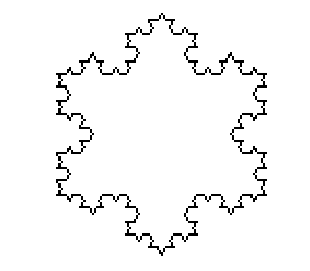
\includegraphics[width=3.5cm, height=3cm]{flocon3.pdf}
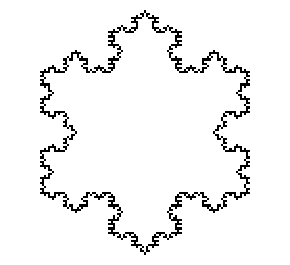
\includegraphics[width=3.5cm, height=3cm]{flocon4.pdf}

\begin{figure}[H]
	\centering
	\caption{Les côtes de la Bretagne}
	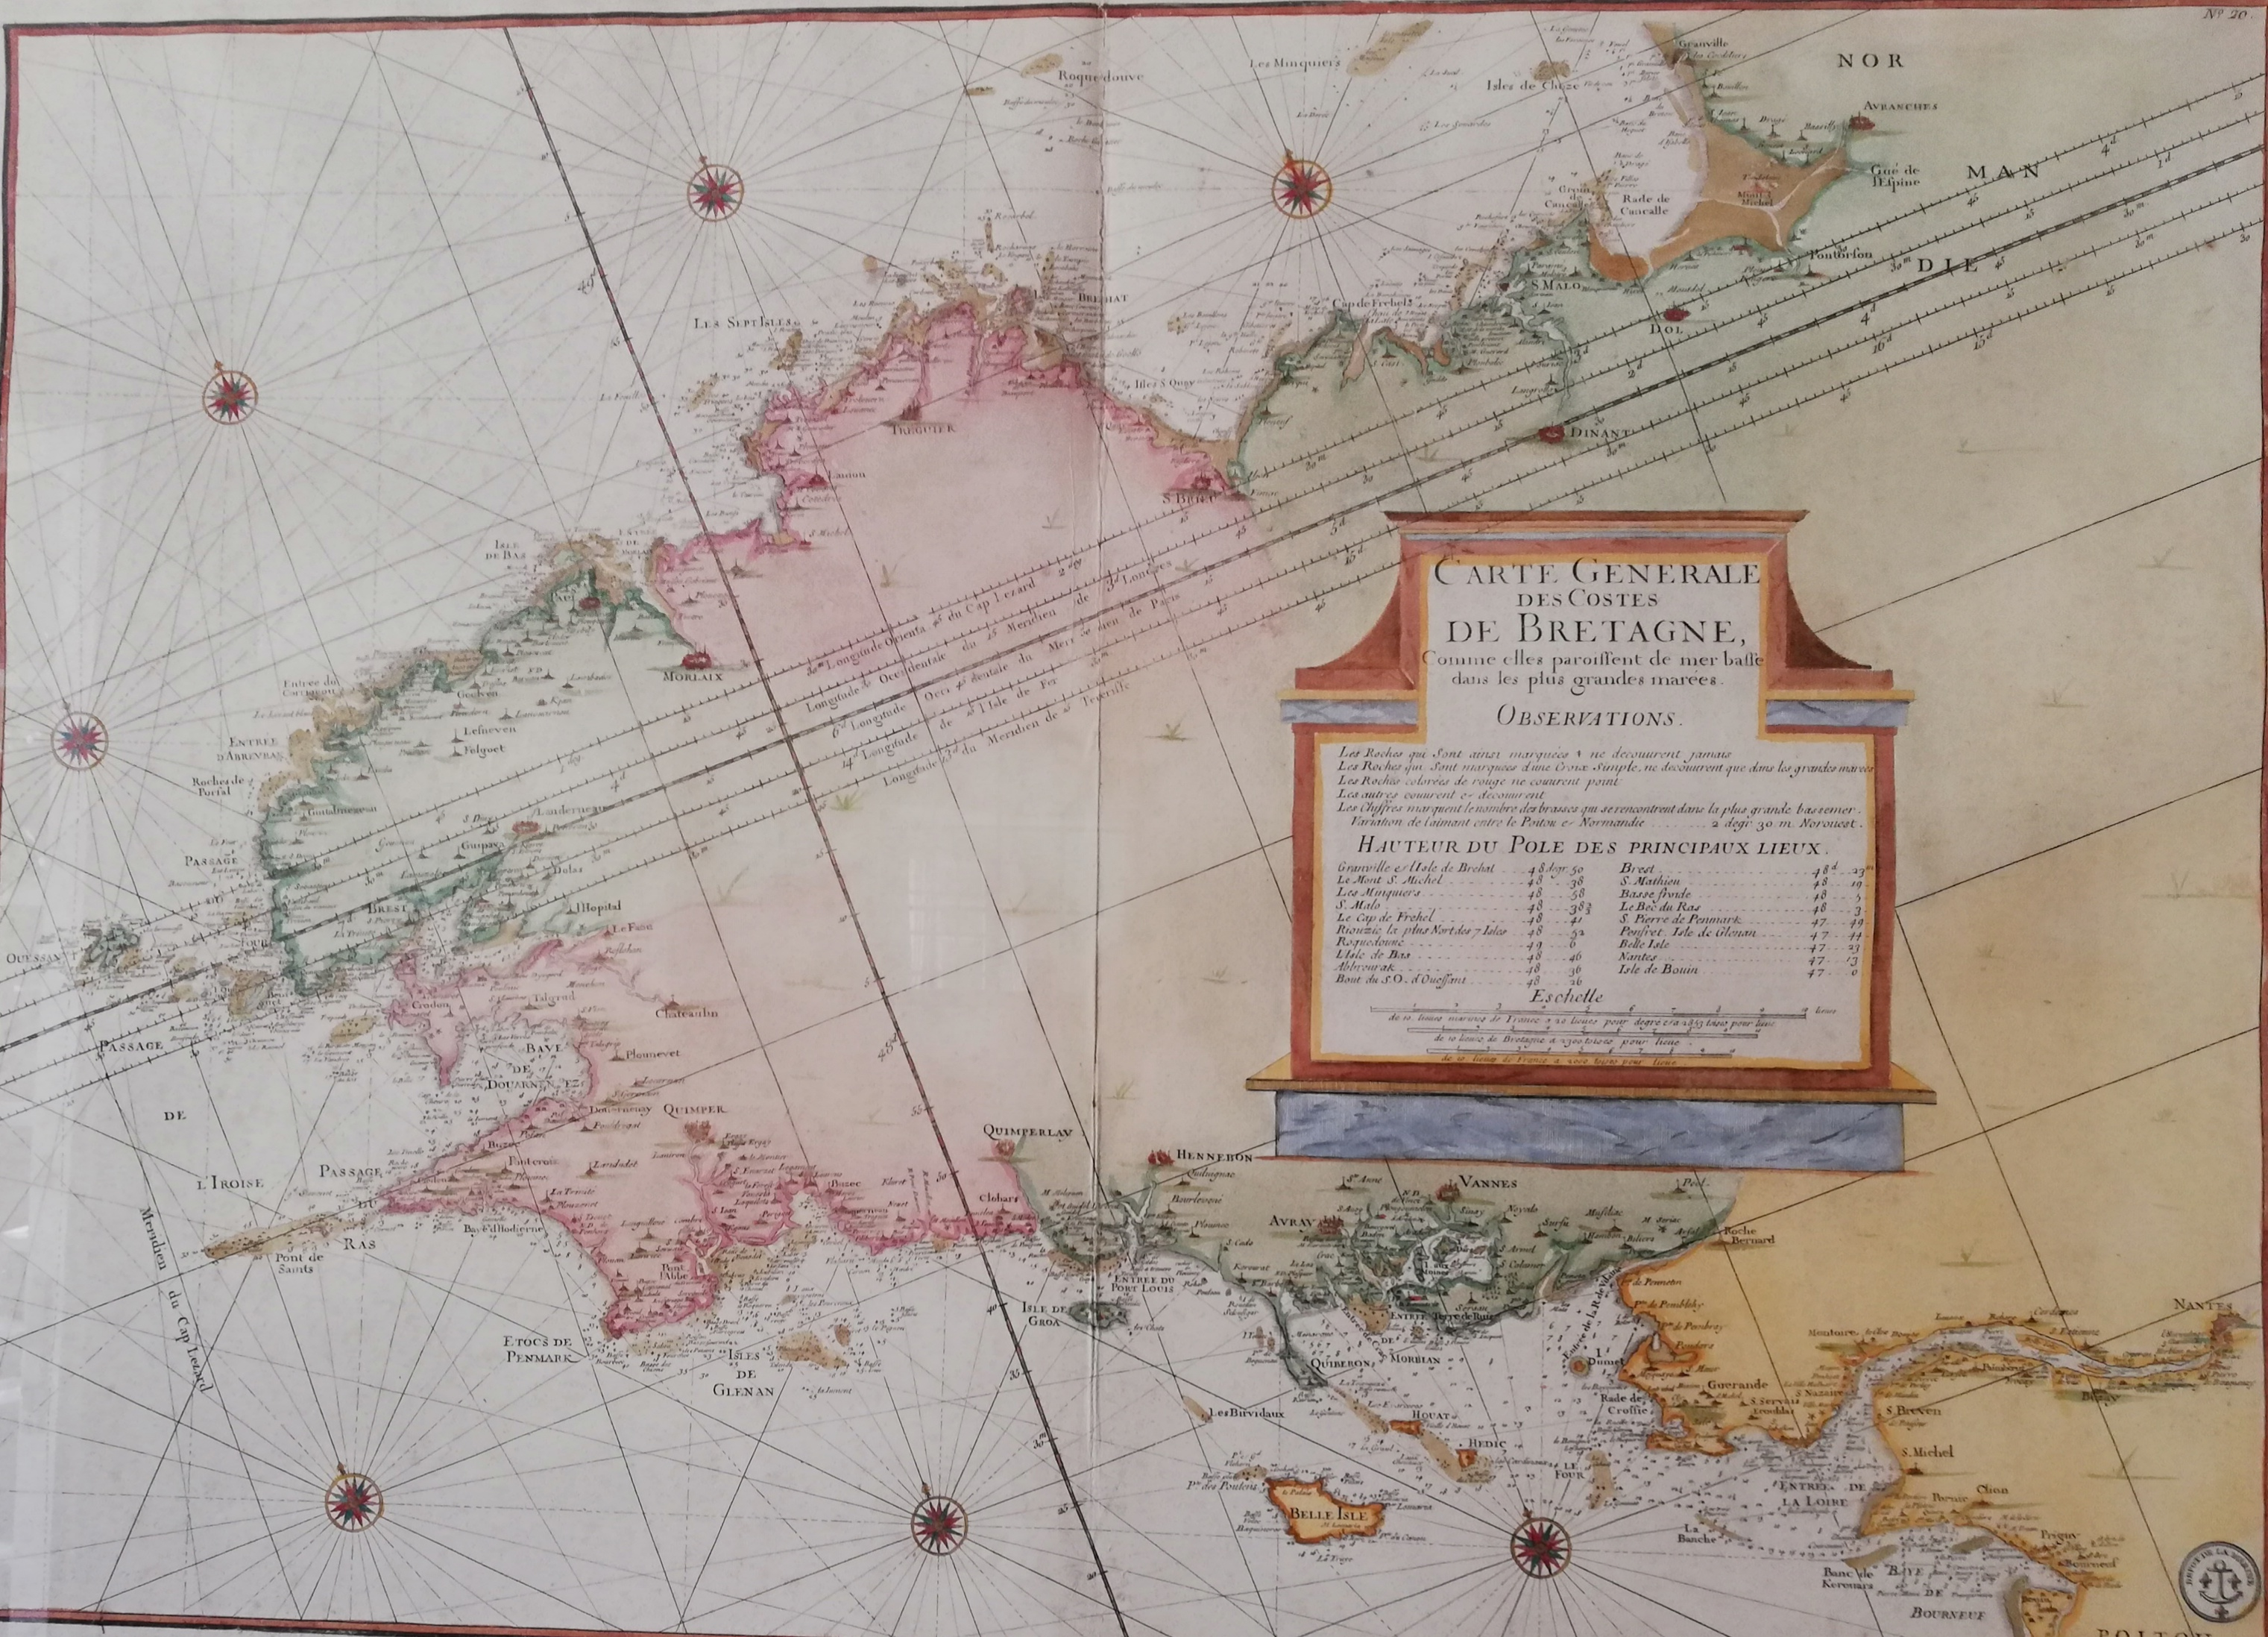
\includegraphics[width=4.0cm]{bretagne.png}
\end{figure}

\section{Utilisation de \MF}
\MF est un langage créé par D. Knuth \cite{mf}. Il permet le
design de nouvelles fontes de manière très élégante sous forme d'équations.
La programmation se fait sous forme principalement déclarative.

Je me suis ici amusé à créer un nouveau petit symbole que vous 
avez dû voir souvent dans cet article: \imp

\section{The boxes}
Nous avons vu comment représenter un environnement comme une liste
d'associations avec des paires \verb+variable.valeur+.
Une autre méthode est d'utiliser le principe de \textit{box} qui encapsule la
valeur dans une lambda. La \textit{box} est une lambda qui prend une valeur à  sa
création. Puis elle réagit à  deux messages qui permettent respectivement
d'afficher la valeur capturée ou de la modifier avec la procédure \verb+set!+


Voici l'implémentation en Scheme:
\begin{Verbatim}
(define (box value)
  (lambda (msg)
    (case msg
      ("get" value)
      ("set" (lambda (new-value) (set! value new-value))))))

(define (make-box value)
  (box value))

(define maboite (make-box 4))
(maboite "get")
((maboite "set") 5)
\end{Verbatim}

En CAML, nous pouvons rédiger le code ci-dessous:
\begin{Verbatim}
exception Erreur

let box value0 =
	let value = ref value0 in
	fun message ->
		match message with
		| "get" -> (fun any -> print_int !value)
		| "set" -> (fun newvalue -> (value := newvalue ; print_int !value ))
		| "reset"-> (fun any -> (value := value0 ; print_int !value))
		| _ -> raise Erreur
		
		
let maboite = box 5 ;;
(maboite "get") 0 ;;
(maboite "set") 1976 ;;
(maboite "get") 0 ;;
(maboite "reset") 0 ;;
\end{Verbatim}

\section{Les modules OCAML. Modélisation d'un monoïde}
Un monoïde est une structure algébrique qui possède une loi de composition
interne associative et un élément neutre.
Représentons cette structure en OCAML, en définissant un module.
Nous reprenons ici l'excellent article 
https://blog.derniercri.io/observons-une-premiere-structure-algebrique-appliquee-a-linformatique-le-monoide/
\begin{Verbatim}
module type MONOID =
sig
type t
val ( <+> ) : t -> t -> t
val neutral : t	
end

module String_monoid : MONOID with type t = string  =
struct
type t = string
let ( <+> ) = (^)
let neutral = ""
end

String_monoid.("abc" <+> "def" <+> neutral)
-> String_monoid.t = "abcdef"	
\end{Verbatim}

En algèbre, un morphisme (ou homomorphisme) est une application entre deux structures algébriques
de même espèce.

Pour les  monoïdes, un morphisme est une application 
$f:(M,*,e)\longrightarrow (M',\star ,e')$ , entre deux monoïdes $ (M,*,e)$ et 
$(M',\star , e')$ qui vérifie :
\begin{itemize}
	\item $\forall (g,h)\in M^{2},~f(g*h)=f(g)\star f(h)$
	\item $f(e)=e'$
\end{itemize}
\begin{Verbatim}
#load "Str.cma"

let count  t =  split (regexp " ") t   |> List.length ;;

let pageA = "Hello World "
let pageB = "Foo bar "
let pageC = "O Caml " ;;

count String_monoid.(pageA <+> pageB <+>  pageC) ;;
count(String_monoid.(pageA)) + count(String_monoid.(pageB)) + count(String_monoid.(pageC));;
\end{Verbatim}
Nous avons ici utilisé l'opérateur \verb+|>+ défini comme suit \verb+let ( |> ) x f = f x+

Cette fonction \verb+count+ est ainsi un morphisme entre le monoïde \verb+String_monoid+ et 
le monoïde des entiers (avec $+$ comme fonction de composition interne et $0$
comme élément neutre)

\section{La machine de Turing}
Une machine de Turing est un automate à  état (\textit{state machine}) qui a la
capacité de lire puis  d'enregistrer un caractère sur une bande de longueur
infinie. 

La machine change d'état sur la base de trois éléments: l'état courant,
le caractère lu de la bande et une table externe de transition. La table de
transition est externe à  la bande et elle est statique.
 L'action résultante est un changement potentiel d'état, une écriture de
 caractère sur la bande et un déplacement à  droite ou à  gauche de la tête de
 lecture.

Nous implémentons cela avec le concept de \textit{box} présenté dans le chapitre
précédent. La lambda va encapsuler l'état courant, la position de la tête de
lecture, la bande et la table de transition.
La table de transition est modélisée par une a-liste d'a-listes.
La première a-liste permet de faire matcher l'état courant.
La seconde a-liste permet de faire matcher le caractère lu.
Ces deux informations combinées fournissent  le triplet de sortie
\verb+(état_suivant, caractère_écrit, direction)+

\begin{Verbatim}
let matable = [ ("q0" , [ (">", ("q1", "X", "G")) ;
								  ("<", ("q0", "<", "D")) ; 
								  (" ", ("q2", " ", "G")) ;
								  ("X", ("q0", "X",	"D")) ]) ;
			       ("q1" , [ (">", ("q1", ">", "G")) ;
			                 ("<", ("q0", "X", "D")) ;
			                 (" ", ("qf", "non", "G")) ;
			                 ("X", ("q1", "X", "G")) ]) ;
			       ("q2" , [ (">", ("q2", ">", "G")) ;
			                 ("<", ("qf", "non", "G")) ;
			                 (" ", ("qf", "oui", "G")) ;
			                 ("X", ("q2", "X", "G")) ]) ;
			   ] ;;
\end{Verbatim}

Cette table de transition va nous permettre de vérifier le bon parenthésage
d'une expression en entrée fournie sur la bande représentée par une liste 
\verb+let mabande =   [" "; "<"; ">"; " "]+

L'état \verb+q0+ va rechercher une parenthèse \verb+>+ en allant vers la droite.

L'état \verb+q1+ va rechercher une parenthèse \verb+<+ en allant vers la gauche.

L'état \verb+q2+ va rechercher une parenthèse \verb+>+ en allant vers la gauche.


Les parenthèses matchées sont remplacées par le caractère \verb+X+.
Le passage à  l'état final \verb+qf+ est accompagné par l'écriture \verb+oui+ ou
\verb+non+ sur la bande suivant si l'expression est ou non correctement parenthésée.

\begin{Verbatim}

let make_turing table etat0 position0 bande0 =
	let etat = ref etat0 in
	let position = ref position0 in
	let bande = ref bande0 in
	let fct_transition state input = assoc input (assoc state table) in
	let lire () = nth !bande !position in
	let deplacer = function 
		| "G" -> if (!position = 0) then (bande := " " :: !bande) else (position := !position - 1) 
    | "D" -> 
	   begin
		  position := !position + 1 ;
		  if ((lire ()) = " ") then (bande := !bande @ (" ":: []))
   	 end
		| _ -> raise Erreur
	in
	let rec liste_tail liste pos =
	  match pos with
	  | 0 -> liste
	  | n -> liste_tail (tl liste) (pos - 1)
  in
  let rec liste_tete liste pos =
	  match pos with
	  | 0 -> []
  	| n -> (hd liste) :: liste_tete (tl liste) (pos - 1)
  in
	let ecrire symb =
	bande := (liste_tete !bande !position) @ (symb :: []) @ ( liste_tail (tl !bande) !position)
	in
	 fun instruction ->
		match instruction with
		| "executer" -> 
			let (e, s, d) = fct_transition !etat (lire ()) in
	    	begin
		      ecrire s ;
		      deplacer d;
		      etat := e ;
					if (!etat = "qf") then raise Final 
	      end 
		| "reset" -> begin etat := etat0 ; bande := bande0; position := position0 end
		| "affiche"  -> 
			   begin print_string "etat:" ; print_string !etat ; 
				       print_string "  position:"; print_int !position ; 
							 print_string "  lire:"; print_string (lire ()) ;
							 print_string "  bande:  "; print_liste !bande
	       end	
		| _ -> raise Erreur
		
let executer_turing turing trace =
	let rec iterer () =
		turing "executer" ; if trace then turing "affiche"; iterer () 
	in
	begin
	 turing "reset" ;
	 try
	  iterer () 
	 with Final -> turing "affiche"
	 end 

\end{Verbatim}

Voici le résultat sur l'expression $ <> $
\begin{Verbatim}
# let turing_par = make_turing matable etatinit posinit  [" "; "<"; ">"; " "]  ;;
# executer_turing turing_par true ;;

etat:q0  position:2  lire:>  bande:   <> 
etat:q1  position:1  lire:<  bande:   <X 
etat:q0  position:2  lire:X  bande:   XX 
etat:q0  position:3  lire:   bande:   XX  
etat:q2  position:2  lire:X  bande:   XX  
etat:q2  position:1  lire:X  bande:   XX  
etat:q2  position:0  lire:   bande:   XX  
etat:qf  position:0  lire:   bande:   ouiXX  
\end{Verbatim}

Et voici le résultat sur l'expression $ <<><> $
\begin{Verbatim}
# let turing_par = make_turing matable etatinit posinit  [" "; "<"; "<"; ">"; "<"; ">"; " "] ;;
# executer_turing turing_par true ;;

etat:q0  position:2  lire:<  bande:   <<><> 
etat:q0  position:3  lire:>  bande:   <<><> 
etat:q1  position:2  lire:<  bande:   <<X<> 
etat:q0  position:3  lire:X  bande:   <XX<> 
etat:q0  position:4  lire:<  bande:   <XX<> 
etat:q0  position:5  lire:>  bande:   <XX<> 
etat:q1  position:4  lire:<  bande:   <XX<X 
etat:q0  position:5  lire:X  bande:   <XXXX 
etat:q0  position:6  lire:   bande:   <XXXX  
etat:q2  position:5  lire:X  bande:   <XXXX  
etat:q2  position:4  lire:X  bande:   <XXXX  
etat:q2  position:3  lire:X  bande:   <XXXX  
etat:q2  position:2  lire:X  bande:   <XXXX  
etat:q2  position:1  lire:<  bande:   <XXXX  
etat:qf  position:0  lire:   bande:   nonXXXX  
\end{Verbatim}

\section{La machine à pile}
Nous utilisons l'implémentation ci-dessous pour la représentation des piles sous
formes de listes mutables.
\begin{Verbatim}
type 'a pile = 'a list ref ;;
let empiler x p = p := x :: !p ;;

exception Vide ;;

let depiler p =  
	match !p with
  | [] -> raise Vide
  |x::t -> p:=t ; x ;;

let sommet p =
	match !p with
	| [] -> raise Vide
	| x::t -> x  ;;
\end{Verbatim}

La machine à pile exécutera les instructions suivantes:\\
\verb+["EMPILER"; "nombre"],["ADD"], ["SUB"], ["MUL"], ["STOP"]+

La lecture d'une instruction est réalisée par la fonction \texttt{fetch}. Cette
fonction parcourt de manière linéaire le code représenté par un \textit{array}.
Chaque \texttt{fetch} incrémente la variable \verb+pc+ qui représente le
\textit{program counter}.

\begin{Verbatim}
exception Erreur ;;
	
let executer code =
	let pc = ref 0 in
	let pile = ref [] in
	let fetch code  =
	begin
		pc := !pc + 1 ; 
		Array.get code (!pc - 1) 
	end 
	in
	let rec exec () =
		let instr = fetch code in
		match instr with
		| ["EMPILER"; n] -> ( empiler (int_of_string n) pile ; exec () )
		| ["ADD"] -> let v2 = depiler pile in let v1 = depiler pile in 
		            ( empiler (v1 + v2) pile ; exec () )
		| ["SUB"] -> let v2 = depiler pile in let v1 = depiler pile in
		            ( empiler (v1 - v2) pile ; exec () )
		| ["MUL"] -> let v2 = depiler pile in let v1 = depiler pile in
		            ( empiler (v1 * v2) pile ; exec () )
		| ["STOP"] -> print_int (sommet pile)
		| _ -> raise Erreur
	in exec ()
\end{Verbatim}

Voici l'exécution de la machine à pile:
\begin{Verbatim}
let code = [| ["EMPILER"; "10"] ;["EMPILER"; "15"] ; ["ADD"] ;
						  ["EMPILER"; "4"] ; ["MUL"] ; ["STOP"] |] ;;
						  
# executer code ;;
# 100- : unit = ()
\end{Verbatim}

\section{Machine Learning and Neural Networks}

\subsection{Introduction}

Nous implémentons en R un réseau de neurones réduit à sa plus simple expression.
Il n'aura que deux couches de neurones.
Le langage R est ici commode pour ses opérations natives sur les matrices.
Nous pourrons voir ensuite comme transposer ce code en OCAML.

Nous entraînerons notre NN sur la base du jeu de test MNIST.
Le  "training set" contient 60000 exemples, et le "test set" 10000 exemples.
Nous pourrons nous documenter plus précisément avec l'excellent ouvrage de François Chollet \cite{deepR}.

\subsection{Un peu de théorie}

Soit les 150 observations suivantes représentées par la matrice $X_{150,784}$ (ou tensor 2 dimensions) comprenant 150 lignes pour les 150 observations et 784 colonnes pour les 784 features des observations.

2 matrices de poids $W^1_{32,150}$ et $W^2_{10,150}$ sont utilisées.

\begin{itemize}
	\item 1er layer de 32 neurones
	\item 2nd layer de 10 neurones
\end{itemize}

La sortie $OUTPUT_{150,10}$ est une matrice de 150 lignes avec les 10 colonnes représentant 
les 10 features que l'on cherche à reconnaître.

Voici le schéma simplifié du NN à 2 couches:

$$
X \longrightarrow \otimes W^1 \rightarrow  Z^1 \rightarrow \sigma \rightarrow LAYER^1 \longrightarrow
\otimes W^2 
\rightarrow Z^2 
\rightarrow 
\sigma 
\rightarrow \hat{Y} 
>> LOSS(\hat{Y}, Y)
$$

\subsection{Calcul matriciel}

Cela donne le calcul matriciel ci-dessous:
\begin{footnotesize}
\begin{align*}
\begin{pmatrix}
x_{1,1} & x_{1,2} & \cdots & x_{1,784} \\
x_{2,1} & x_{2,2} & \cdots & x_{2,784} \\
\vdots  & \vdots  & \ddots & \vdots  \\
x_{150,1} & x_{150,2} & \cdots & x_{150,784} 
\end{pmatrix}
\times
\begin{pmatrix}caml
w^1_{1,1} & w^1_{1,2} & \cdots & w^1_{1,32} \\
w^1_{2,1} & w^1_{2,2} & \cdots & w^1_{2,32} \\
\vdots  & \vdots  & \ddots & \vdots  \\
w^1_{784,1} & w^1_{784,2} & \cdots & w^1_{784,32} 
\end{pmatrix}
&= 
\begin{pmatrix}
z^1_{1,1} & z^1_{1,2} & \cdots & z^1_{1,32} \\
z^1_{2,1} & z^1_{2,2} & \cdots & z^1_{2,32} \\
\vdots  & \vdots  & \ddots & \vdots  \\
z^1_{150,1} & z^1_{150,2} & \cdots & z^1_{150,32} 
\end{pmatrix}
\\
\sigma(
\begin{pmatrix}
z^1_{1,1} & z^1_{1,2} & \cdots & z^1_{1,32} \\
z^1_{2,1} & z^1_{2,2} & \cdots & z^1_{2,32} \\
\vdots  & \vdots  & \ddots & \vdots  \\
z^1_{150,1} & z^1_{150,2} & \cdots & z^1_{150,32} 
\end{pmatrix}
)
\times
\begin{pmatrix}
w^2_{1,1} & w^2_{1,2} & \cdots & w^2_{1,10} \\
w^2_{2,1} & w^2_{2,2} & \cdots & w^2_{2,n} \\
\vdots  & \vdots  & \ddots & \vdots  \\
w^2_{32,1} & w^2_{32,2} & \cdots & w^2_{32,10} 
\end{pmatrix}
&= 
\begin{pmatrix}
z^2_{1,1} & z^2_{1,2} & \cdots & z^2_{1,10} \\
z^2_{2,1} & z^2_{2,2} & \cdots & z^2_{2,10} \\
\vdots  & \vdots  & \ddots & \vdots  \\
z^2_{150,1} & z^2_{150,2} & \cdots & z^2_{150,10} 
\end{pmatrix}
\\
\sigma(
\begin{pmatrix}
z^2_{1,1} & z^2_{1,2} & \cdots & z^2_{1,10} \\
z^2_{2,1} & z^2_{2,2} & \cdots & z^2_{2,10} \\
\vdots  & \vdots  & \ddots & \vdots  \\
z^2_{150,1} & z^2_{150,2} & \cdots & z^2_{150,10}
\end{pmatrix}
)
&=
\begin{pmatrix}
\hat{y}_{1,1} & \hat{y}_{1,2} & \cdots & \hat{y}_{1,10} \\
\hat{y}_{2,1} & \hat{y}_{2,2} & \cdots & \hat{y}_{2,10} \\
\vdots  & \vdots  & \ddots & \vdots  \\
\hat{y}_{150,1} & \hat{y}_{150,2} & \cdots & \hat{y}_{150,10} 
\end{pmatrix}
\end{align*}
\begin{align*}
LOSS(Y, \hat{Y}) &= \sum (
\begin{pmatrix}
\hat{y}_{1,1} & \hat{y}_{1,2} & \cdots & \hat{y}_{1,10} \\
\hat{y}_{2,1} & \hat{y}_{2,2} & \cdots & \hat{y}_{2,10} \\
\vdots  & \vdots  & \ddots & \vdots  \\
\hat{y}_{150,1} & \hat{y}_{150,2} & \cdots & \hat{y}_{150,10} 
\end{pmatrix}
-
\begin{pmatrix}
y_{1,1} & y_{1,2} & \cdots & y_{1,10} \\
y_{2,1} & y_{2,2} & \cdots & y_{2,10} \\
\vdots  & \vdots  & \ddots & \vdots  \\
y_{150,1} & y_{150,2} & \cdots & y_{150,10} 
\end{pmatrix}
)^2
\end{align*}

\begin{align*}
Z_1 &= X.W_1 \\
LAYER_1 &= \sigma (Z_1) \\
Z_2 &= LAYER_1 * W_2 \\
\hat{Y} &= \sigma (Z_2) \\
LOSS &= (\hat{Y} -Y)^2  
\end{align*}
\end{footnotesize}

Calculons la dérivée de la fonction $LOSS$ en fonction de $W^1$

\begin{align*}
 \frac{\delta LOSS}{\delta W_1} &=\frac{\delta LOSS}{\delta \hat{Y}} . \frac{\delta \hat{Y}}{\delta Z_2}. \frac{\delta Z_2}{\delta LAYER_1 }.\frac{\delta LAYER_1}{\delta Z_1 }. \frac{\delta Z_1}{\delta W_1 } \\ 
  &= 2(\hat{Y}-Y) . \sigma ^\prime (Z_2) . W_2 . \sigma ^\prime (Z_1). X
\end{align*}

$2(\hat{Y}-Y)$ est une matrice de dimension $(150, 10)$

$\sigma ^\prime (Z_2)$ est une matrice de dimension $(150,10)$

$W_2$ est une matrice de dimension $(32,10)$

$\sigma ^\prime (Z_1)$ est une matrice de dimension $(150,32)$

$X$ est une matrice de dimension $(150,784)$

Le calcul matriciel qui sera fait est $t(X)* \{ (2(\hat{Y}-Y) . \sigma ^\prime (Z^2) * t(W^2). \sigma ^\prime (Z^1)\}$, où $*$ est le produit matriciel et $.$ le produit d'Hadamard.
Le résultat donne une matrice de dimension $(784,32)$ qui est de même dimension que $W_1$
\begin{align*}
t(150,784)* \{(150,10).(150,10)*t(32,10).(150,32))\} &= (784,150) * \{(150,10)*(10,32).(150,32)\}\\ 
&= (784,150)*(150,32) \\
&=(784,32)
\end{align*}

 
\subsection{Fonctions d'activation}

Pour la fonction d'activation, ici appelée $\sigma$, nous utiliserons pour la première couche la fonction $relu(x) = max(o,x)$

Pour la seconde couche, nous utiliserons la fonction sigmoid $f(x)= \frac{1}{1+e^{-x}}$

\begin{figure}[H]
\centering
\caption{La fonction sigmoid}
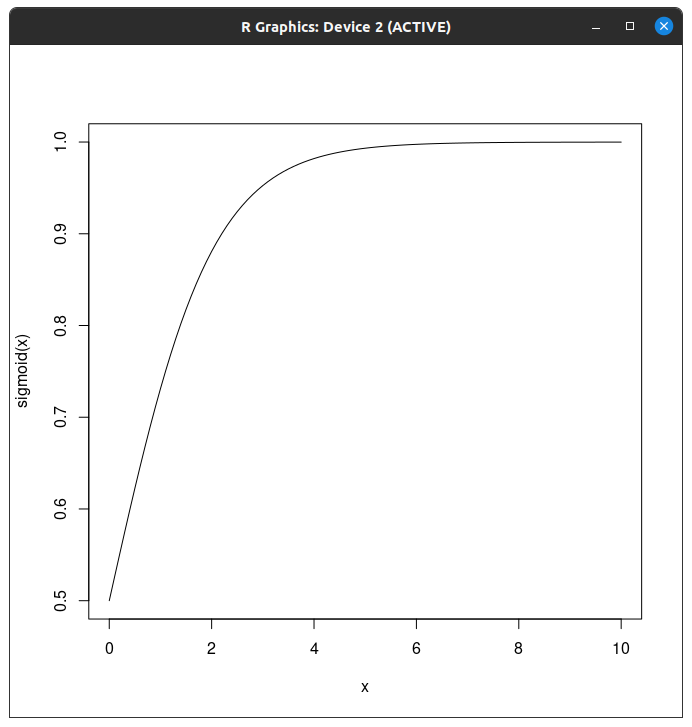
\includegraphics[width=5cm, height=5cm]{sigmoid}
\end{figure}

Voici le code en R:

\begin{Verbatim}
# the activation function
sigmoid <- function(x) {
	1.0 / (1.0 + exp(-x))
}

x=seq(0,10,0.1)
plot(x, sigmoid(x), type="l") 

# the derivative of the activation function
sigmoid_derivative <- function(x) {
	sigmoid(x) * (1.0 - sigmoid(x))
}
\end{Verbatim}


Calculons la dérivée de la fonction $LOSS$ en fonction de $W^2$ 

\begin{align}
\frac{\delta LOSS}{\delta W_2} & =\frac{\delta LOSS}{\delta \hat{Y}} . \frac{\delta \hat{Y}}{\delta Z_2}. \frac{\delta Z_2}{\delta W_2 } \\
 &= 2(\hat{Y}-Y) . \sigma ^\prime (Z_2) . LAYER_1 
\end{align}

$2(\hat{Y}-Y)$ est une matrice de dimension $(150, 10)$

$\sigma ^\prime (Z_2)$ est une matrice de dimension $(150,10)$

$LAYER_1$ est une matrice de dimension $(150,32)$

Le calcul matriciel qui sera fait est $t(LAYER_1)* (2(\hat{Y}-Y) . \sigma ^\prime (Z_2))$, où $*$ est le produit matriciel et $.$ le produit d'Hadamard.
Le résultat donne une matrice de dimension $(32,10)$ qui est de même dimension que $W_2$
$$
t(150,32) * (150,10).(150.10) = (32,150)*(150,10)=(32,10)
$$

\section{Poésies}
\begin{verse}
	Un soir t'en souvient-il ? Nous voguions en silence ; \\
	On n’entendait au loin, sur l’onde et sous les cieux,  \\
	Que le bruit des rameurs qui frappaient en cadence     \\
	Tes flots harmonieux. \\
\end{verse}
\begin{verse}
	Les feuilles mortes se ramassent à la pelle \\
	Tu vois, je n'ai pas oublié... \\
	Les feuilles mortes se ramassent à la pelle, \\
	Les souvenirs et les regrets aussi \\
\end{verse}

\section{Les nombres premiers}

\begin{itemize}
	\item Le crible d'Erathostene
	\item Leur répartition
	\item Les nombres premiers jumeaux
	\item La constante de Brun 
	\item La fonction zêta
	\item Le produit eulérien et sa convergence avec la suite harmonique
\end{itemize}


\subsection{Le produit d'Euler aka le produit eulérien}
La fonction zêta est égale au produit eulérien
\[ \zeta(s) = \sum_{n=1}^{\infty} \frac{1}{n^s} = \prod_{i=1}^\infty \frac{1}{1-p_i^{-s}} = \prod_{i=1}^\infty \frac{p_i^s}{p_i^s-1} \]

Exemple pour $s=1$ avec la suite harmonique
$$
\begin{array}{ccc}
1+ \frac{1}{2} + \frac{1}{3} + \frac{1}{4} + \frac{1}{5} +...  &=  \frac{1}{1-\frac{1}{2}} .\frac{1}{1-\frac{1}{3}}.\frac{1}{1-\frac{1}{5}}.\frac{1}{1-\frac{1}{7}}. (...) \\[\bigskipamount]
&= \frac{2.3.5.7.11.13.17.19...}{1.2.4.6.10.12.16.18...} 
\end{array}
$$

Démontrons cela
\[\zeta(1) = 1+ \frac{1}{2} + \frac{1}{3} + \frac{1}{4} + \frac{1}{5}+ \frac{1}{6}+ \frac{1}{7} +  \frac{1}{8} +... \]

Divisons par 2
\[ \frac{\zeta(1)}{2} = \frac{1}{2}+\frac{1}{4}+\frac{1}{6}+\frac{1}{8}+\frac{1}{10}+\frac{1}{12} + \frac{1}{14}+ \frac{1}{16}+... \]
 
La différence de ces 2 équations donne:
\[ \zeta(1).(1-\frac{1}{2}) = 1 + \frac{1}{3}+\frac{1}{5}+\frac{1}{7}+\frac{1}{9}+\frac{1}{11}+\frac{1}{13}+ ... \]

Divisons par 3
\[ \frac{1}{3}.(1-\frac{1}{2}).\zeta(1) = \frac{1}{3} + \frac{1}{9}+\frac{1}{15}+\frac{1}{21}+\frac{1}{27}+ \frac{1}{33}+ \frac{1}{39}+... \]

La différence donne:
\[ (1-\frac{1}{3}).(1-\frac{1}{2}).\zeta(1) = 1 + \frac{1}{5} + \frac{1}{7}+\frac{1}{11}+\frac{1}{13}+ ... \]

Divisons par 5
\[ \frac{1}{5}.(1-\frac{1}{3}).(1-\frac{1}{2}).\zeta(1) =    \frac{1}{5} + \frac{1}{25}+\frac{1}{35}+\frac{1}{55}+ ... \]

La différence donne:
\[(1-\frac{1}{5}).(1-\frac{1}{3}).(1-\frac{1}{2}).\zeta(1) = 1 + \frac{1}{7}+\frac{1}{11}+\frac{1}{13}+... \]

Nous pouvons poursuivre sur le principe du crible d'Erathostène
\[ \ldots(1-\frac{1}{5}).(1-\frac{1}{3}).(1-\frac{1}{2}).\zeta(1) = 1 \]

D'où :
$$
\begin{array}{ccc}
\zeta(1) &=& \frac{1}{(1-\frac{1}{2}).(1-\frac{1}{3}).(1-\frac{1}{5})\ldots} \\[\bigskipamount]
\zeta(1) &=& \frac{1}{\frac{1}{2}.\frac{2}{3}.\frac{4}{5}\ldots} 		\\[\bigskipamount]
\zeta(1) &=&  \frac{2.3.5.7.11.13.17.19...}{1.2.4.6.10.12.16.18...} \\[\bigskipamount]
\end{array}
$$

Le numérateur est le produit de l'ensemble des nombres premiers.
Le dénominateur est le produit de l'ensemble des nombres premiers moins 1.


Exemple pour $s=2$ avec la suite carrée
\[ 1+ \frac{1}{4} + \frac{1}{9} + \frac{1}{16} + ...  =  \frac{1}{1-\frac{1}{4}} .\frac{1}{1-\frac{1}{9}}.\frac{1}{1-\frac{1}{25}}.\frac{1}{1-\frac{1}{49}}. (...) \]



\subsection{Les nombres premiers jumeaux et la constante de Brun}
La somme inverse des nombres premiers jumeaux. Il y en aurait une infinité. Cependant, cette somme
 converge vers la constante de Brun.

\[ Brun = (\frac{1}{3} + \frac{1}{5}) + (\frac{1}{5} + \frac{1}{7}) + (\frac{1}{11} + \frac{1}{13}) + (\frac{1}{17} + \frac{1}{19}) + (\frac{1}{29} + \frac{1}{31}) +\  ... \]

\[ Brun \approx 1,90216 \]


\section{L'alphabet grec. Extraits du nouveau testament}
\[
\begin{array}{cccccccccccccccccccccccc}
 \alpha & \beta &\gamma &  \delta & \epsilon & \zeta & \eta &\theta & \iota &\kappa &\lambda & \mu & \nu & \xi & o & \pi & \rho & \sigma & \tau & 
 \upsilon & \phi & \chi & \psi & \omega \\
 A & B & \Gamma & \Delta & E & Z & H & \Theta & I & K & \Lambda & M & N  &\Xi & O & \Pi & R & \Sigma & T & \Upsilon & \Phi & X & \Psi & \Omega
 \end{array}
 \]

 \textgreek{	
Ἐγὼ τὸ Ἄλφα  καὶ τὸ Omega, ὁ  πρῶτος καὶ ὁ ἔσχατος, ἡ ἀρχὴ καὶ τὸ τέλος

Ἄλλην παραβολὴν παρέθηκεν αὐτοῖς, λέγων, Ὁμοία ἐστὶν ἡ βασιλεία τῶν οὐρανῶν
κόκκῳ σινάπεως, ὃν λαβὼν ἄνθρωπος ἔσπειρεν ἐν τῷ ἀγρῷ αὐτοῦ:
ὃ μικρότερον μέν ἐστιν πάντων τῶν σπερμάτων: ὅταν δὲ αὐξηθῇ,
μεῖζον τῶν λαχάνων ἐστίν, καὶ γίνεται δένδρον, ὥστε ἐλθεῖν τὰ πετεινὰ τοῦ οὐρανοῦ 
καὶ κατασκηνοῦν ἐν τοῖς κλάδοις αὐτοῦ.

Eirene umin !
}

\bibliographystyle{plain}
\bibliography{book}

\end{document}
